%%
% Copyright (c) 2017 - 2023, Pascal Wagler;
% Copyright (c) 2014 - 2023, John MacFarlane
%
% All rights reserved.
%
% Redistribution and use in source and binary forms, with or without
% modification, are permitted provided that the following conditions
% are met:
%
% - Redistributions of source code must retain the above copyright
% notice, this list of conditions and the following disclaimer.
%
% - Redistributions in binary form must reproduce the above copyright
% notice, this list of conditions and the following disclaimer in the
% documentation and/or other materials provided with the distribution.
%
% - Neither the name of John MacFarlane nor the names of other
% contributors may be used to endorse or promote products derived
% from this software without specific prior written permission.
%
% THIS SOFTWARE IS PROVIDED BY THE COPYRIGHT HOLDERS AND CONTRIBUTORS
% "AS IS" AND ANY EXPRESS OR IMPLIED WARRANTIES, INCLUDING, BUT NOT
% LIMITED TO, THE IMPLIED WARRANTIES OF MERCHANTABILITY AND FITNESS
% FOR A PARTICULAR PURPOSE ARE DISCLAIMED. IN NO EVENT SHALL THE
% COPYRIGHT OWNER OR CONTRIBUTORS BE LIABLE FOR ANY DIRECT, INDIRECT,
% INCIDENTAL, SPECIAL, EXEMPLARY, OR CONSEQUENTIAL DAMAGES (INCLUDING,
% BUT NOT LIMITED TO, PROCUREMENT OF SUBSTITUTE GOODS OR SERVICES;
% LOSS OF USE, DATA, OR PROFITS; OR BUSINESS INTERRUPTION) HOWEVER
% CAUSED AND ON ANY THEORY OF LIABILITY, WHETHER IN CONTRACT, STRICT
% LIABILITY, OR TORT (INCLUDING NEGLIGENCE OR OTHERWISE) ARISING IN
% ANY WAY OUT OF THE USE OF THIS SOFTWARE, EVEN IF ADVISED OF THE
% POSSIBILITY OF SUCH DAMAGE.
%%

%%
% This is the Eisvogel pandoc LaTeX template.
%
% For usage information and examples visit the official GitHub page:
% https://github.com/Wandmalfarbe/pandoc-latex-template
%%

% Options for packages loaded elsewhere
\PassOptionsToPackage{unicode}{hyperref}
\PassOptionsToPackage{hyphens}{url}
\PassOptionsToPackage{dvipsnames,svgnames,x11names,table}{xcolor}
%
\documentclass[
  paper=a4,
  ,captions=tableheading
]{scrartcl}
\usepackage{amsmath,amssymb}
% Use setspace anyway because we change the default line spacing.
% The spacing is changed early to affect the titlepage and the TOC.
\usepackage{setspace}
%\setstretch{1.2}
\setstretch{1.0}
\usepackage{iftex}
\ifPDFTeX
  \usepackage[T1]{fontenc}
  \usepackage[utf8]{inputenc}
  \usepackage{textcomp} % provide euro and other symbols
\else % if luatex or xetex
  \usepackage{unicode-math} % this also loads fontspec
  \defaultfontfeatures{Scale=MatchLowercase}
  \defaultfontfeatures[\rmfamily]{Ligatures=TeX,Scale=1}
\fi
\usepackage{lmodern}
\ifPDFTeX\else
  % xetex/luatex font selection
\fi
% Use upquote if available, for straight quotes in verbatim environments
\IfFileExists{upquote.sty}{\usepackage{upquote}}{}
\IfFileExists{microtype.sty}{% use microtype if available
  \usepackage[]{microtype}
  \UseMicrotypeSet[protrusion]{basicmath} % disable protrusion for tt fonts
}{}
\makeatletter
\@ifundefined{KOMAClassName}{% if non-KOMA class
  \IfFileExists{parskip.sty}{%
    \usepackage{parskip}
  }{% else
    \setlength{\parindent}{0pt}
    \setlength{\parskip}{6pt plus 2pt minus 1pt}}
}{% if KOMA class
  \KOMAoptions{parskip=half}
  % adjust appearance of footnotes, start:
  \deffootnote{1em}{0em}{%
    \textsuperscript{\thefootnotemark}%
    \setlength{\parskip}{\baselineskip}%
    \setlength{\parindent}{0pt}%
    }
  }
  % adjust appearance of footnotes, end.
\makeatother
\usepackage{xcolor}
\definecolor{default-linkcolor}{HTML}{A50000}
\definecolor{default-filecolor}{HTML}{A50000}
\definecolor{default-citecolor}{HTML}{4077C0}
\definecolor{default-urlcolor}{HTML}{4077C0}
\usepackage[margin=2.5cm,includehead=true,includefoot=true,centering,]{geometry}
\usepackage{color}
\usepackage{fancyvrb}
\newcommand{\VerbBar}{|}
\newcommand{\VERB}{\Verb[commandchars=\\\{\}]}
\DefineVerbatimEnvironment{Highlighting}{Verbatim}{commandchars=\\\{\}}
% Add ',fontsize=\small' for more characters per line
\usepackage{framed}
\definecolor{shadecolor}{RGB}{248,248,248}
\newenvironment{Shaded}{\begin{snugshade}}{\end{snugshade}}
\newcommand{\AlertTok}[1]{\textcolor[rgb]{0.94,0.16,0.16}{#1}}
\newcommand{\AnnotationTok}[1]{\textcolor[rgb]{0.56,0.35,0.01}{\textbf{\textit{#1}}}}
\newcommand{\AttributeTok}[1]{\textcolor[rgb]{0.13,0.29,0.53}{#1}}
\newcommand{\BaseNTok}[1]{\textcolor[rgb]{0.00,0.00,0.81}{#1}}
\newcommand{\BuiltInTok}[1]{#1}
\newcommand{\CharTok}[1]{\textcolor[rgb]{0.31,0.60,0.02}{#1}}
\newcommand{\CommentTok}[1]{\textcolor[rgb]{0.56,0.35,0.01}{\textit{#1}}}
\newcommand{\CommentVarTok}[1]{\textcolor[rgb]{0.56,0.35,0.01}{\textbf{\textit{#1}}}}
\newcommand{\ConstantTok}[1]{\textcolor[rgb]{0.56,0.35,0.01}{#1}}
\newcommand{\ControlFlowTok}[1]{\textcolor[rgb]{0.13,0.29,0.53}{\textbf{#1}}}
\newcommand{\DataTypeTok}[1]{\textcolor[rgb]{0.13,0.29,0.53}{#1}}
\newcommand{\DecValTok}[1]{\textcolor[rgb]{0.00,0.00,0.81}{#1}}
\newcommand{\DocumentationTok}[1]{\textcolor[rgb]{0.56,0.35,0.01}{\textbf{\textit{#1}}}}
\newcommand{\ErrorTok}[1]{\textcolor[rgb]{0.64,0.00,0.00}{\textbf{#1}}}
\newcommand{\ExtensionTok}[1]{#1}
\newcommand{\FloatTok}[1]{\textcolor[rgb]{0.00,0.00,0.81}{#1}}
\newcommand{\FunctionTok}[1]{\textcolor[rgb]{0.13,0.29,0.53}{\textbf{#1}}}
\newcommand{\ImportTok}[1]{#1}
\newcommand{\InformationTok}[1]{\textcolor[rgb]{0.56,0.35,0.01}{\textbf{\textit{#1}}}}
\newcommand{\KeywordTok}[1]{\textcolor[rgb]{0.13,0.29,0.53}{\textbf{#1}}}
\newcommand{\NormalTok}[1]{#1}
\newcommand{\OperatorTok}[1]{\textcolor[rgb]{0.81,0.36,0.00}{\textbf{#1}}}
\newcommand{\OtherTok}[1]{\textcolor[rgb]{0.56,0.35,0.01}{#1}}
\newcommand{\PreprocessorTok}[1]{\textcolor[rgb]{0.56,0.35,0.01}{\textit{#1}}}
\newcommand{\RegionMarkerTok}[1]{#1}
\newcommand{\SpecialCharTok}[1]{\textcolor[rgb]{0.81,0.36,0.00}{\textbf{#1}}}
\newcommand{\SpecialStringTok}[1]{\textcolor[rgb]{0.31,0.60,0.02}{#1}}
\newcommand{\StringTok}[1]{\textcolor[rgb]{0.31,0.60,0.02}{#1}}
\newcommand{\VariableTok}[1]{\textcolor[rgb]{0.00,0.00,0.00}{#1}}
\newcommand{\VerbatimStringTok}[1]{\textcolor[rgb]{0.31,0.60,0.02}{#1}}
\newcommand{\WarningTok}[1]{\textcolor[rgb]{0.56,0.35,0.01}{\textbf{\textit{#1}}}}

% Workaround/bugfix from jannick0.
% See https://github.com/jgm/pandoc/issues/4302#issuecomment-360669013)
% or https://github.com/Wandmalfarbe/pandoc-latex-template/issues/2
%
% Redefine the verbatim environment 'Highlighting' to break long lines (with
% the help of fvextra). Redefinition is necessary because it is unlikely that
% pandoc includes fvextra in the default template.
\usepackage{fvextra}
\DefineVerbatimEnvironment{Highlighting}{Verbatim}{breaklines,fontsize=\small,commandchars=\\\{\}}

\usepackage{longtable,booktabs,array}
\usepackage{calc} % for calculating minipage widths
% Correct order of tables after \paragraph or \subparagraph
\usepackage{etoolbox}
\makeatletter
\patchcmd\longtable{\par}{\if@noskipsec\mbox{}\fi\par}{}{}
\makeatother
% Allow footnotes in longtable head/foot
\IfFileExists{footnotehyper.sty}{\usepackage{footnotehyper}}{\usepackage{footnote}}
\makesavenoteenv{longtable}
% add backlinks to footnote references, cf. https://tex.stackexchange.com/questions/302266/make-footnote-clickable-both-ways
\usepackage{footnotebackref}
\usepackage{graphicx}
\makeatletter
\def\maxwidth{\ifdim\Gin@nat@width>\linewidth\linewidth\else\Gin@nat@width\fi}
\def\maxheight{\ifdim\Gin@nat@height>\textheight\textheight\else\Gin@nat@height\fi}
\makeatother
% Scale images if necessary, so that they will not overflow the page
% margins by default, and it is still possible to overwrite the defaults
% using explicit options in \includegraphics[width, height, ...]{}
\setkeys{Gin}{width=\maxwidth,height=\maxheight,keepaspectratio}
% Set default figure placement to htbp
\makeatletter
% Make use of float-package and set default placement for figures to H.
% The option H means 'PUT IT HERE' (as  opposed to the standard h option which means 'You may put it here if you like').
\usepackage{float}
\floatplacement{figure}{H}
\makeatother
\setlength{\emergencystretch}{3em} % prevent overfull lines
\providecommand{\tightlist}{%
  \setlength{\itemsep}{0pt}\setlength{\parskip}{0pt}}
\setcounter{secnumdepth}{5}
\ifLuaTeX
  \usepackage{selnolig}  % disable illegal ligatures
\fi
\IfFileExists{bookmark.sty}{\usepackage{bookmark}}{\usepackage{hyperref}}
\IfFileExists{xurl.sty}{\usepackage{xurl}}{} % add URL line breaks if available
\urlstyle{same}
\hypersetup{
  pdftitle={Putting Fortran's object-related features to practical use},
  pdfauthor={Reinhold Bader (1966--2024)},
  pdfkeywords={Fortran, OOP},
  colorlinks=true,
  linkcolor={blue},
  filecolor={default-filecolor},
  citecolor={default-citecolor},
  urlcolor={default-urlcolor},
  breaklinks=true,
  pdfcreator={LaTeX via pandoc with an edited Eisvogel template}}
\title{Putting Fortran's object-related features to practical use}
\author{Reinhold Bader (1966--2024)}
\date{2024}



%%
%% added
%%


%
% for the background color of the title page
%

%
% break urls
%
\PassOptionsToPackage{hyphens}{url}

%
% When using babel or polyglossia with biblatex, loading csquotes is recommended
% to ensure that quoted texts are typeset according to the rules of your main language.
%
\usepackage{csquotes}

%
% captions
%
\definecolor{caption-color}{HTML}{777777}
\usepackage[font={stretch=1.2}, textfont={color=caption-color}, position=top, skip=4mm, labelfont=bf, singlelinecheck=false, justification=raggedright]{caption}
\setcapindent{0em}

%
% blockquote
%
\definecolor{blockquote-border}{RGB}{221,221,221}
\definecolor{blockquote-text}{RGB}{119,119,119}
\usepackage{mdframed}
\newmdenv[rightline=false,bottomline=false,topline=false,linewidth=3pt,linecolor=blockquote-border,skipabove=\parskip]{customblockquote}
\renewenvironment{quote}{\begin{customblockquote}\list{}{\rightmargin=0em\leftmargin=0em}%
\item\relax\color{blockquote-text}\ignorespaces}{\unskip\unskip\endlist\end{customblockquote}}

%
% Source Sans Pro as the default font family
% Source Code Pro for monospace text
%
% 'default' option sets the default
% font family to Source Sans Pro, not \sfdefault.
%
\ifnum 0\ifxetex 1\fi\ifluatex 1\fi=0 % if pdftex
    % \usepackage[default]{sourcesanspro}
  % \usepackage{sourcecodepro}
  \usepackage{libertine}
  \usepackage{libertinust1math}
  \usepackage[scaled=0.84]{beramono}
  \renewcommand*{\figureformat}{}
  \else % if not pdftex
    \usepackage[default]{sourcesanspro}
  \usepackage{sourcecodepro}

  % XeLaTeX specific adjustments for straight quotes: https://tex.stackexchange.com/a/354887
  % This issue is already fixed (see https://github.com/silkeh/latex-sourcecodepro/pull/5) but the
  % fix is still unreleased.
  % TODO: Remove this workaround when the new version of sourcecodepro is released on CTAN.
  \ifxetex
    \makeatletter
    \defaultfontfeatures[\ttfamily]
      { Numbers   = \sourcecodepro@figurestyle,
        Scale     = \SourceCodePro@scale,
        Extension = .otf }
    \setmonofont
      [ UprightFont    = *-\sourcecodepro@regstyle,
        ItalicFont     = *-\sourcecodepro@regstyle It,
        BoldFont       = *-\sourcecodepro@boldstyle,
        BoldItalicFont = *-\sourcecodepro@boldstyle It ]
      {SourceCodePro}
    \makeatother
  \fi
  \fi

%
% heading color
%
\definecolor{heading-color}{RGB}{40,40,40}
\addtokomafont{section}{\color{heading-color}}
% When using the classes report, scrreprt, book,
% scrbook or memoir, uncomment the following line.
%\addtokomafont{chapter}{\color{heading-color}}

%
% variables for title, author and date
%
\usepackage{titling}
\title{Putting Fortran's object-related features to practical use}
\author{Reinhold Bader (1966--2024)}
\date{2024}

%
% tables
%

\definecolor{table-row-color}{HTML}{F5F5F5}
\definecolor{table-rule-color}{HTML}{999999}

%\arrayrulecolor{black!40}
\arrayrulecolor{table-rule-color}     % color of \toprule, \midrule, \bottomrule
\setlength\heavyrulewidth{0.3ex}      % thickness of \toprule, \bottomrule
\renewcommand{\arraystretch}{1.3}     % spacing (padding)


%
% remove paragraph indentation
%
\setlength{\parindent}{0pt}
\setlength{\parskip}{6pt plus 2pt minus 1pt}
\setlength{\emergencystretch}{3em}  % prevent overfull lines

%
%
% Listings
%
%


%
% header and footer
%
\usepackage[headsepline,footsepline]{scrlayer-scrpage}

\newpairofpagestyles{eisvogel-header-footer}{
  \clearpairofpagestyles
  \ihead*{Putting Fortran's object-related features to practical use}
  \chead*{}
  \ohead*{2024}
  \ifoot*{Reinhold Bader (1966--2024)}
  \cfoot*{}
  \ofoot*{\thepage}
  \addtokomafont{pageheadfoot}{\upshape}
}
\pagestyle{eisvogel-header-footer}



%%
%% end added
%%

\begin{document}

%%
%% begin titlepage
%%

%%
%% end titlepage
%%

% \maketitle


{
\hypersetup{linkcolor=}
\setcounter{tocdepth}{3}
\tableofcontents
}
This article by the late Reinhold Bader (1966-2024) describes how
advanced Fortran language features can be applied toward object-based
and object-oriented programming techniques. These are, of course, to a
significant extent a matter of taste, personal style and possibly
overarching program design considerations, so should be taken with a
pinch of salt.

Language features from Fortran 95 and later will be used; those from
Fortran 2003 and later will also be shortly described. They are
explained in more detail in e.g., Metcalf, Reid, Cohen and
Bader.\footnote{Metcalf, Michael; Reid, John; Cohen, Malcolm; Bader,
  Reinhold (2023). \emph{Modern Fortran Explained.} Numerical
  Mathematics and Scientific Computation. Oxford University Press.
  \href{https://en.wikipedia.org/wiki/Special:BookSources/978-0-19-887657-1}{ISBN
  978-0-19-887657-1}.} See also
\href{https://en.wikipedia.org/wiki/Fortran_95_language_features}{Fortran
95 language features} for the language's fundamentals; the prerequisite
for understanding this article is that features explained there are well
understood.

Boldface will be used where term definitions are introduced. They are
additionally annotated by ``(not a Fortran term)'' or similar if the
term is not used in the Fortran standard itself, but is in general use
in the technical literature.

Compilable and runnable example code is available from an external
\href{https://github.com/reinh-bader/object_fortran}{Github repository}.

\section{Object-based programming techniques}\label{sec:oop_techniques}

\subsection{Introduction: Container-like
types}\label{introduction-container-like-types}

The word ``Container-like'' is not a Fortran term, but used in the
context of this article to designate types with components whose size
(or type, to be discussed later) is not known when the type is declared.
For deferred sizing of array objects, this can be achieved by using
either the \texttt{pointer} or the \texttt{allocatable} attribute for
the component's specification.

The language features and programming techniques will be shown using two
examples introduced in the following section. The demonstration codes
for this chapter can be found in the \texttt{object\_based} folder of
the \href{https://github.com/reinh-bader/object_fortran}{Github
repository}.

\subsection{Examples for definitions of container-like
types}\label{examples-for-definitions-of-container-like-types}

\subsubsection{Allocatable components}\label{allocatable-components}

As an example for the type definition of a \textbf{value container} (not
a Fortran term) with an \texttt{ALLOCATABLE} component consider

\begin{Shaded}
\begin{Highlighting}[]
\DataTypeTok{type} \DataTypeTok{::}\NormalTok{ polynomial}
  \DataTypeTok{private}
  \DataTypeTok{real}\NormalTok{, }\DataTypeTok{allocatable} \DataTypeTok{::}\NormalTok{ a(:)}
\DataTypeTok{end type}
\end{Highlighting}
\end{Shaded}

An object declared to be of this type

\begin{Shaded}
\begin{Highlighting}[]
\DataTypeTok{type(polynomial)} \DataTypeTok{::}\NormalTok{ p}
\end{Highlighting}
\end{Shaded}

is suitable for characterization of a polynomial

\(p(x) = \sum_{k=0}^{\text{degree}} a_{k} \cdot x^k \quad (x \in \Re)\)

once it has been created and subsequently supplied with values of the
coefficients:

\begin{Shaded}
\begin{Highlighting}[]
\NormalTok{degree }\KeywordTok{=}\NormalTok{ ... }\CommentTok{! integer value known at run time only}
\KeywordTok{allocate}\NormalTok{( p}\OperatorTok{\%}\NormalTok{a(}\DecValTok{0}\NormalTok{:degree) )}
\NormalTok{p}\OperatorTok{\%}\NormalTok{a(}\DecValTok{0}\NormalTok{:) }\KeywordTok{=}\NormalTok{ ...}
\end{Highlighting}
\end{Shaded}

\subsubsection{Pointer components}\label{pointer-components}

As an example for the type definition of a \textbf{reference container}
(not a Fortran term) with a \texttt{POINTER} component consider

\begin{Shaded}
\begin{Highlighting}[]
\DataTypeTok{type} \DataTypeTok{::}\NormalTok{ sorted\_list}
  \DataTypeTok{private}
  \DataTypeTok{type(sortable)} \DataTypeTok{::}\NormalTok{ data}
  \DataTypeTok{type(sorted\_list)}\NormalTok{, }\DataTypeTok{pointer} \DataTypeTok{::}\NormalTok{ next }\KeywordTok{=}\OperatorTok{\textgreater{}}\NormalTok{ null()}
\DataTypeTok{end type}
\end{Highlighting}
\end{Shaded}

Note that referencing the type itself when declaring a component is
permitted if that component has the \texttt{pointer} or
\texttt{allocatable} attribute; such types are generally known as
\textbf{recursive}. They are used to represent information structures
(lists, trees, \ldots), often with specific relationships between the
individual data entries stored in each node. In this example, the
assumption is that entries of type \texttt{data} in subsequent list
items fulfill an ordering condition, based on the functionality supplied
with that type:

\begin{Shaded}
\begin{Highlighting}[]
\DataTypeTok{type}\NormalTok{, }\DataTypeTok{public} \DataTypeTok{::}\NormalTok{ sortable}
  \DataTypeTok{character(len=:)}\NormalTok{, }\DataTypeTok{allocatable} \DataTypeTok{::}\NormalTok{ string}
\DataTypeTok{end type}

\KeywordTok{interface} \KeywordTok{operator}\NormalTok{(}\OperatorTok{\textless{}}\NormalTok{)         }\CommentTok{! compare two objects of type sortable}
  \KeywordTok{module procedure}\NormalTok{ less\_than  }\CommentTok{! implementation not shown here}
\KeywordTok{end interface}
\end{Highlighting}
\end{Shaded}

\emph{Hint:} Given that Fortran supports arrays, use of simple linked
lists is in most cases inappropriate. The example is presented here as
being the simplest that permits illustrating the language features of
interest.

An object declared to be

\begin{Shaded}
\begin{Highlighting}[]
\DataTypeTok{type(sorted\_list)} \DataTypeTok{::}\NormalTok{ my\_list}
\end{Highlighting}
\end{Shaded}

is suitable as starting point for building a linked list with node
entries of type \texttt{data}. In the simplest case, inserting a data
item into the object is done by executing the following statements:

\begin{Shaded}
\begin{Highlighting}[]
\DataTypeTok{type(sortable)} \DataTypeTok{::}\NormalTok{ my\_data}
\NormalTok{:}
\NormalTok{my\_data }\KeywordTok{=}\NormalTok{ ...}
\NormalTok{my\_list}\OperatorTok{\%}\NormalTok{data }\KeywordTok{=}\NormalTok{ my\_data  }\CommentTok{! only compiles if type definition is accessible in host}
\end{Highlighting}
\end{Shaded}

However, as we shall see below, setting up a complete and valid
\texttt{sorted\_list} object in a reliable manner needs additional work.

\subsection{Constructing objects of container-like
type}\label{constructing-objects-of-container-like-type}

The semantics of the default structure constructor for container-like
objects needs to account for any additional \texttt{pointer} or
\texttt{allocatable} attribute specified for type components.

For the first example type from the last section, the executable
statements in

\begin{Shaded}
\begin{Highlighting}[]
\DataTypeTok{type(polynomial)} \DataTypeTok{::}\NormalTok{ q, r}
\NormalTok{:}
\NormalTok{q }\KeywordTok{=}\NormalTok{ polynomial( }\KeywordTok{[}\FloatTok{2.}\NormalTok{, }\FloatTok{3.}\NormalTok{, }\FloatTok{1.}\KeywordTok{]}\NormalTok{ )}
\NormalTok{r }\KeywordTok{=}\NormalTok{ polynomial( null() )}
\end{Highlighting}
\end{Shaded}

result in an object \texttt{q} auto-allocated to the value
\texttt{q\%a(1:3)\ ==\ {[}2.,\ 3.,\ 1.{]}}, and an object \texttt{r}
with \texttt{r\%a} unallocated.

For the second example type from the last section, the executable
statements in

\begin{Shaded}
\begin{Highlighting}[]
\DataTypeTok{type(sorted\_list)} \DataTypeTok{::}\NormalTok{ sl1}
\DataTypeTok{type(sorted\_list)}\NormalTok{, }\DataTypeTok{target} \DataTypeTok{::}\NormalTok{ sl2}
\DataTypeTok{type(sortable)} \DataTypeTok{::}\NormalTok{ d1, d2}
\NormalTok{:}
\NormalTok{sl1 }\KeywordTok{=}\NormalTok{ sorted\_list( data}\KeywordTok{=}\NormalTok{d1, next}\KeywordTok{=}\NormalTok{sl2 )  }\CommentTok{! use keyword notation}
\NormalTok{sl2 }\KeywordTok{=}\NormalTok{ sorted\_list( d2, null() )}
\end{Highlighting}
\end{Shaded}

result in an object \texttt{sl1} with \texttt{sl1\%next} pointer
associated with \texttt{sl2}, and an object \texttt{sl2} with
\texttt{sl2\%next} disassociated; the \texttt{data} components of both
objects have values, \texttt{d1} and \texttt{d2}, respectively. Note
that an argument that matches with a \texttt{pointer} component must
have either the \texttt{pointer} or the \texttt{target} attribute. Also,
\textbf{keyword notation} can be used in structure constructors in the
same manner as for procedure arguments.

The default constructor's behaviour has some properties that one needs
to be aware of:

\begin{enumerate}
\def\labelenumi{\arabic{enumi}.}
\tightlist
\item
  If all type components have the \texttt{private} attribute i.e., the
  type is \textbf{opaque} (not a Fortran term), it can only be used if
  the type declaration is accessed by host association (this is the same
  as for nonallocatable/nonpointer components);
\item
  especially for container-like types, its semantics may be incompatible
  with the programmers intentions for how the objects should be used.
\end{enumerate}

Item 2 is illustrated by the above object setups, specifically:

\begin{itemize}
\tightlist
\item
  In the \texttt{polynomial} example given above, the lower bound of
  \texttt{q\%a} is set to 1, contrary to the expectation that it should
  be 0. One could account for this by calculating index offsets in any
  module procedures that process \texttt{polynomial} objects, but this
  makes the code harder to understand and maintain. Also, the degree of
  the polynomial should be determined by the last nonzero entry of the
  coefficient array, but the language can of course not be aware of
  this.
\item
  In the \texttt{sorted\_list} example given above, the ordering
  requirement for entries in subsequent nodes is not checked, so will
  usually be not fulfilled. Also, if \texttt{sl2} goes out of scope
  before \texttt{sl1} does, the list structure is torn to bits.
\end{itemize}

The programmer can enforce appropriate semantics by overloading the
structure constructor. In this case, it is usually a good idea to
declare the types as being opaque.

Overloading the structure constructor is done by

\begin{itemize}
\tightlist
\item
  creating a named interface (i.e., a generic function) with the same
  name as the type of interest;
\item
  creating at least one specific function (a subroutine is not
  permitted), usually returning a scalar result of the type of interest.
\end{itemize}

For the \texttt{polynomial} type the interface block (placed in the
specification section of the module containing the type definition)
might read

\begin{Shaded}
\begin{Highlighting}[]
\KeywordTok{interface}\NormalTok{ polynomial}
\CommentTok{! overload to assure correct lower bound when creating a polynomial object}
  \KeywordTok{module procedure} \DataTypeTok{::}\NormalTok{ create\_polynomial}
\NormalTok{  ... }\CommentTok{! further specifics as needed}
\KeywordTok{end interface}
\end{Highlighting}
\end{Shaded}

and the implementation of \texttt{create\_polynomial} (in the
\texttt{contains} part of the module) might read

\begin{Shaded}
\begin{Highlighting}[]
\KeywordTok{pure} \DataTypeTok{type(polynomial)} \KeywordTok{function}\NormalTok{ create\_polynomial(a)}
  \DataTypeTok{real}\NormalTok{, }\DataTypeTok{intent(in)} \DataTypeTok{::}\NormalTok{ a(}\DecValTok{0}\NormalTok{:)}
  \DataTypeTok{integer} \DataTypeTok{::}\NormalTok{ degree(}\DecValTok{1}\NormalTok{)}

\NormalTok{  degree }\KeywordTok{=} \FunctionTok{findloc}\NormalTok{( a }\OperatorTok{/=} \FloatTok{0.0}\NormalTok{, }\DataTypeTok{value}\KeywordTok{=}\ConstantTok{.true.}\NormalTok{, back}\KeywordTok{=}\ConstantTok{.true.}\NormalTok{ ) }\KeywordTok{{-}} \DecValTok{1}
  \KeywordTok{allocate}\NormalTok{( create\_polynomial}\OperatorTok{\%}\NormalTok{a(}\DecValTok{0}\NormalTok{:degree(}\DecValTok{1}\NormalTok{)) )}
\NormalTok{  create\_polynomial}\OperatorTok{\%}\NormalTok{a(}\DecValTok{0}\NormalTok{:) }\KeywordTok{=}\NormalTok{ a(}\DecValTok{0}\NormalTok{:degree(}\DecValTok{1}\NormalTok{))}
\KeywordTok{end function}
\end{Highlighting}
\end{Shaded}

Because its signature matches the default structure constructor's, the
function actually overrides the default constructor, making it generally
unavailable.

For the \texttt{sorted\_list} type the interface block might read

\begin{Shaded}
\begin{Highlighting}[]
\KeywordTok{interface}\NormalTok{ sorted\_list}
\CommentTok{! the default constructor is unavailable because the type is opaque}
\CommentTok{! the specific has a different signature than the structure constructor}
  \KeywordTok{module procedure} \DataTypeTok{::}\NormalTok{ create\_sorted\_list}
\NormalTok{  ... }\CommentTok{! further specifics as needed}
\KeywordTok{end interface}
\end{Highlighting}
\end{Shaded}

with the implementation of \texttt{create\_sorted\_list} as follows:

\begin{Shaded}
\begin{Highlighting}[]
\KeywordTok{pure} \KeywordTok{function}\NormalTok{ create\_sorted\_list(item\_array) }\KeywordTok{result}\NormalTok{(head)}
  \DataTypeTok{type(sortable)}\NormalTok{, }\DataTypeTok{intent(in)} \DataTypeTok{::}\NormalTok{ item\_array(:)}
  \DataTypeTok{type(sorted\_list)} \DataTypeTok{::}\NormalTok{ head}
  \DataTypeTok{integer} \DataTypeTok{::}\NormalTok{ i}

  \KeywordTok{do}\NormalTok{ i }\KeywordTok{=} \DecValTok{1}\NormalTok{, }\FunctionTok{size}\NormalTok{(item\_array)}
    \KeywordTok{call}\NormalTok{ add\_to\_sorted\_list(head, item\_array(i))}
    \CommentTok{! handles tedious details of pointer fiddling}
  \KeywordTok{end do}
\KeywordTok{end function}
\end{Highlighting}
\end{Shaded}

The constructor has a signature that differs from that of the default
one, but the latter is unavailable outside the host scope of the type
definition anyway, due to the opacity of \texttt{sorted\_list}.

\subsection{Copying objects of container-like
type}\label{copying-objects-of-container-like-type}

Default assignment extends to container-like objects. For objects
declared as

\begin{Shaded}
\begin{Highlighting}[]
\DataTypeTok{TYPE(polynomial)} \DataTypeTok{::}\NormalTok{ p, q}
\DataTypeTok{TYPE(sorted\_list)} \DataTypeTok{::}\NormalTok{ slp, slq}

\NormalTok{... }\CommentTok{! code that defines p, slp}
\end{Highlighting}
\end{Shaded}

and after defining values for prospective right-hand sides, execution of
the statement

\begin{Shaded}
\begin{Highlighting}[]
\NormalTok{q }\KeywordTok{=}\NormalTok{ p}
\end{Highlighting}
\end{Shaded}

produces the same result as

\begin{Shaded}
\begin{Highlighting}[]
\KeywordTok{if}\NormalTok{ ( }\FunctionTok{allocated}\NormalTok{(q}\OperatorTok{\%}\NormalTok{a) ) }\KeywordTok{deallocate}\NormalTok{( q}\OperatorTok{\%}\NormalTok{a )}
\NormalTok{q}\OperatorTok{\%}\NormalTok{a }\KeywordTok{=}\NormalTok{ p}\OperatorTok{\%}\NormalTok{a  }\CommentTok{! performs auto{-}allocation using the RHS\textquotesingle{}s bounds, then copies the value}
\end{Highlighting}
\end{Shaded}

and execution of the statement

\begin{Shaded}
\begin{Highlighting}[]
\NormalTok{slq }\KeywordTok{=}\NormalTok{ slp}
\end{Highlighting}
\end{Shaded}

produces the same result as

\begin{Shaded}
\begin{Highlighting}[]
\NormalTok{slq}\OperatorTok{\%}\NormalTok{data }\KeywordTok{=}\NormalTok{ slp}\OperatorTok{\%}\NormalTok{data}
\NormalTok{slq}\OperatorTok{\%}\NormalTok{next }\KeywordTok{=}\OperatorTok{\textgreater{}}\NormalTok{ slp}\OperatorTok{\%}\NormalTok{next  }\CommentTok{! creates a reference between list objects without copying any value}
\end{Highlighting}
\end{Shaded}

The terms \textbf{deep copy} and \textbf{shallow copy} (neither are
Fortran terms) are sometimes used to describe the above behaviour for
\texttt{allocatable} and \texttt{pointer} components, respectively. Note
that - different from the default structure constructor - having
\texttt{private} components does not affect the use of default
assigment. However, the semantics of default assignment might not be
what is needed from the programmer's point of view.

Specifically, consider the case where the object \texttt{slq} above has
previously been set up by invoking the overloaded constructor. The
assignment above would then have the following effects:

\begin{enumerate}
\def\labelenumi{\arabic{enumi}.}
\tightlist
\item
  The list elements of the original \texttt{slq}, beginning with
  \texttt{slq\%next}, would become inaccessible (``orphaned''),
  effectively causing a memory leak;
\item
  after the assignment statement, \texttt{slq\%next} references into
  \texttt{slp\%next}, resulting in aliasing.
\end{enumerate}

To avoid 2., it is possible to
\href{https://en.wikipedia.org/wiki/Fortran_95_language_features\#Derived-data_types}{\textbf{overload}
the assignment operator} for reference containers to create a deep copy.
Note that in the case where defined unary or binary operations are
introduced, the functions that define these need to create deep copies
to create the result variable anyway, otherwise things simply don't
work. The downside of this is that in code like

\begin{Shaded}
\begin{Highlighting}[]
\NormalTok{slq }\KeywordTok{=}\NormalTok{ slp }\KeywordTok{//}\NormalTok{ slq}
\end{Highlighting}
\end{Shaded}

~-- with the overloaded concatenation operator meaning that the argument
lists are joined -- multiple deep copies need to be done (the
implementation of the module procedure \texttt{join\_lists} that
supplies the necessary specific for \texttt{//} is not shown here; see
the source \texttt{code\ sorted\_list.f90} for details). It turns out
that some of these exist only intermediately.

Here an implementation of the specific procedure for the overloaded
assignment of \texttt{sorted\_list} objects:

\begin{Shaded}
\begin{Highlighting}[]
\KeywordTok{subroutine}\NormalTok{ assign\_sorted\_list(}\KeywordTok{to}\NormalTok{, from)}
  \DataTypeTok{type(sorted\_list)}\NormalTok{, }\DataTypeTok{intent(in)}\NormalTok{, }\DataTypeTok{target} \DataTypeTok{::}\NormalTok{ from}
  \DataTypeTok{type(sorted\_list)}\NormalTok{, }\DataTypeTok{intent(out)}\NormalTok{, }\DataTypeTok{target} \DataTypeTok{::} \KeywordTok{to}  \CommentTok{! finalizer is executed on entry,}
                                                \CommentTok{! see below for discussion of this.}
  \DataTypeTok{type(sorted\_list)}\NormalTok{, }\DataTypeTok{pointer} \DataTypeTok{::}\NormalTok{ p, q}

\NormalTok{  p }\KeywordTok{=}\OperatorTok{\textgreater{}}\NormalTok{ from; q }\KeywordTok{=}\OperatorTok{\textgreater{}} \KeywordTok{to}

\NormalTok{  deep\_copy : }\KeywordTok{do}
    \KeywordTok{if}\NormalTok{ ( }\FunctionTok{associated}\NormalTok{(p) ) }\KeywordTok{then}
\NormalTok{      q}\OperatorTok{\%}\NormalTok{data }\KeywordTok{=}\NormalTok{ p}\OperatorTok{\%}\NormalTok{data}
    \KeywordTok{else}
      \KeywordTok{exit}\NormalTok{ deep\_copy}
    \KeywordTok{end if}
\NormalTok{    p }\KeywordTok{=}\OperatorTok{\textgreater{}}\NormalTok{ p}\OperatorTok{\%}\NormalTok{next}
    \KeywordTok{if}\NormalTok{ ( }\FunctionTok{associated}\NormalTok{(p) ) }\KeywordTok{allocate}\NormalTok{( q}\OperatorTok{\%}\NormalTok{next )}
\NormalTok{    q }\KeywordTok{=}\OperatorTok{\textgreater{}}\NormalTok{ q}\OperatorTok{\%}\NormalTok{next}
  \KeywordTok{end do}\NormalTok{ deep\_copy}
\KeywordTok{end subroutine}
\end{Highlighting}
\end{Shaded}

Avoiding 1. is usually done by means of finalizers, to be discussed in
the next section. This is because assignment is not the only possible
cause for orphaning of \texttt{pointer}-related memory (or indeed other
resource leaks).

\subsection{Finalization and
conclusions}\label{finalization-and-conclusions}

To deal with resource leaks that are otherwise not within the
programmer's means to avoid, a type definition can be connected with a
user-defined \textbf{final procedure} that is automatically invoked in
certain situations. For the \texttt{sorted\_list} type, this would look
like

\begin{Shaded}
\begin{Highlighting}[]
\DataTypeTok{type} \DataTypeTok{::}\NormalTok{ sorted\_list}
  \DataTypeTok{private}
  \DataTypeTok{type(sortable)} \DataTypeTok{::}\NormalTok{ data}
  \DataTypeTok{type(sorted\_list)}\NormalTok{, }\DataTypeTok{pointer} \DataTypeTok{::}\NormalTok{ next }\KeywordTok{=}\OperatorTok{\textgreater{}}\NormalTok{ null()}
\KeywordTok{contains}
  \DataTypeTok{final} \DataTypeTok{::}\NormalTok{ delete\_sorted\_list}
\DataTypeTok{end type}
\end{Highlighting}
\end{Shaded}

note that the \texttt{final} statement appears after a \texttt{contains}
statement in the type definition; this implies that
\texttt{delete\_sorted\_list} is not a regular type component. The
module procedure's implementation might then be as follows:

\begin{Shaded}
\begin{Highlighting}[]
\KeywordTok{pure} \KeywordTok{recursive} \KeywordTok{subroutine}\NormalTok{ delete\_sorted\_list(list)}
  \DataTypeTok{type(sorted\_list)}\NormalTok{, }\DataTypeTok{intent(inout)} \DataTypeTok{::}\NormalTok{ list}

  \KeywordTok{if}\NormalTok{ ( }\FunctionTok{associated}\NormalTok{(list}\OperatorTok{\%}\NormalTok{next) ) }\KeywordTok{then}
    \KeywordTok{deallocate}\NormalTok{( list}\OperatorTok{\%}\NormalTok{next )  }\CommentTok{! invokes the finalizer recursively}
  \KeywordTok{end if}
\KeywordTok{end subroutine}
\end{Highlighting}
\end{Shaded}

It must be a subroutine that takes a single argument of the type to be
finalized. Most additional attributes are not permitted for that dummy
argument; for the case of finalizing array arguments it is possible to
have a set of finalizers (all listed in the type definition), each of
which declares the dummy argument with an appropriate rank.

\emph{Hint:} The \texttt{pure} and \texttt{recursive} properties
specified above reflect the specific needs for the \texttt{sorted\_list}
type and its associated procedures. The \texttt{recursive} specification
is optional (i.e., procedures can be called recursively by default), but
a \texttt{non\_recursive} specification can be supplied if the
implementation's semantics does not permit correct behaviour in
recursive calls.

The finalizer will be automatically invoked on an object if

\begin{enumerate}
\def\labelenumi{\arabic{enumi}.}
\tightlist
\item
  it appears on the left-hand side of an intrinsic assignment statement
  (before the assignment is performed),
\item
  on invocation of a procedure call where it is argument associated with
  an \texttt{intent(out)} dummy,
\item
  it is a non-saved variable and program execution ends its scope, or
\item
  it is deallocated.
\end{enumerate}

Nonpointer nonallocatable function results fall into the third category
above; however, finalization does not apply for the default structure
constructor.

Note that if a finalizer is defined and the constructor is overloaded,
but the assignment operator is \emph{not}, then the assignment statement
\texttt{slq\ =\ sorted\_list(...)} (which then translates into a single
function call to the \texttt{create\_sorted\_list()} function shown
earlier) will result in a mutilated left-hand side, because the
finalizer will be executed on the function that overloads the
constructor, resulting in \texttt{slq\%next} being disassociated. For
this reason, the following guideline applies:

\begin{quote}
Recommendation:\\
Finalizers, overloads for the default constructor, and overload of the
assignment operation should usually be jointly implemented.
\end{quote}

See also the article
``\href{https://en.wikipedia.org/wiki/Rule_of_three_(C\%2B\%2B_programming)}{Rule
of three}'' for the analogous situation in C++.

\subsection{Further language features useful for object-based
programming}\label{further-language-features-useful-for-object-based-programming}

\subsubsection{Extended semantics for allocatable
objects}\label{extended-semantics-for-allocatable-objects}

Scalars can have the \texttt{allocatable} attribute:

\begin{Shaded}
\begin{Highlighting}[]
\DataTypeTok{character(len=:)}\NormalTok{, }\DataTypeTok{allocatable} \DataTypeTok{::}\NormalTok{ my\_string}
\DataTypeTok{type(sorted\_list)}\NormalTok{, }\DataTypeTok{allocatable} \DataTypeTok{::}\NormalTok{ my\_list}
\end{Highlighting}
\end{Shaded}

Allocation then can be done explicitly; the following examples
illustrate applications of the \texttt{allocate} statement that are
useful or even necessary in this context:

\begin{Shaded}
\begin{Highlighting}[]
\KeywordTok{allocate}\NormalTok{( }\DataTypeTok{character(len=13)} \DataTypeTok{::}\NormalTok{ my\_string )                  }\CommentTok{! typed allocation}
\KeywordTok{allocate}\NormalTok{( my\_list, source}\KeywordTok{=}\NormalTok{sorted\_list(array\_of\_sortable) )  }\CommentTok{! sourced allocation}
\end{Highlighting}
\end{Shaded}

\textbf{Typed allocation} is necessary for the string variable, because
the length parameter of a string is part of its type; we will later see
that derived types can also appear in the type specification.
\textbf{Sourced allocation} permits the creation of an allocated object
that is a clone of the specified source object or expression.

Alternatively, allocatable objects (be they scalar or arrays) can be
auto-allocated by appearing on the left-hand side of an \emph{intrinsic}
assignment statement:

\begin{Shaded}
\begin{Highlighting}[]
\NormalTok{my\_string }\KeywordTok{=} \StringTok{"anything goes"}  \CommentTok{! auto{-}allocated to RHS length before value is transferred}
\CommentTok{! my\_list = sorted\_list(array\_of\_sortable)}
\CommentTok{! the above statement would fail for an unallocated object, because the assignment}
\CommentTok{! has been overloaded using a nonallocatable first dummy argument}
\end{Highlighting}
\end{Shaded}

A caveat is that for \emph{overloaded} assignment, this will usually not
work - either one needs to explicitly allocate the object before
assigning to it, or sourced allocation must be used, which bypasses the
overloaded assignment.

Note that for allocatable objects with deferred-size entries (e.g.,
strings, arrays) a non-conformable left-hand side in an assignment
statement will be deallocated before being allocated to the right length
or shape, respectively.

\emph{Hint:} The features discussed in this subsection are also useful
for object-oriented programming, with additional semantics applying for
the case of polymorphic objects.

\subsubsection{Implementing move
semantics}\label{implementing-move-semantics}

Sometimes it may be necessary to make use of move instead of copy
semantics i.e., create a copy of an object and then getting rid of the
original. The simplest way of doing this is to make use of allocatable
(scalar or array) objects,

\begin{Shaded}
\begin{Highlighting}[]
\DataTypeTok{type(sorted\_list)}\NormalTok{, }\DataTypeTok{allocatable} \DataTypeTok{::}\NormalTok{ my\_list, your\_list}
\end{Highlighting}
\end{Shaded}

After \texttt{your\_list} has been set up, the object's content can then
be transferred to \texttt{my\_list} by using the \texttt{move\_alloc}
intrinsic,

\begin{Shaded}
\begin{Highlighting}[]
\KeywordTok{call}\NormalTok{ move\_alloc(your\_list, my\_list)}
\end{Highlighting}
\end{Shaded}

which will deallocate \texttt{my\_list} if necessary, before doing the
transfer. After the invocation, \texttt{my\_list} will have the value
formerly stored in \texttt{your\_list}, and \texttt{your\_list} will end
up in the deallocated state. Note that the latter does not involve a
regular object deallocation (effectively, a descriptor for the object is
moved), so any existing finalizer will not be invoked.

\subsubsection{\texorpdfstring{The \texttt{block}
construct}{The block construct}}\label{the-block-construct}

The above rules on finalization imply that variables declared in the
specification part of the main program are not finalizable, since they
by default have the \texttt{save} attribute. One could argue this is not
necessary since all assigned memory is reclaimed when program execution
ends. However, excessive memory consumption or the use of other
resources may cause issues for reliable program execution. To work
around these, the \texttt{block} construct can be used:

\begin{Shaded}
\begin{Highlighting}[]
\KeywordTok{program}\NormalTok{ test\_sorted\_list}
  \KeywordTok{use}\NormalTok{ mod\_sortable}
  \KeywordTok{use}\NormalTok{ mod\_sorted\_list}
  \KeywordTok{implicit} \KeywordTok{none}
\NormalTok{  :}
\NormalTok{  work : }\KeywordTok{block}
    \DataTypeTok{type(sortable)} \DataTypeTok{::}\NormalTok{ array(items)}
    \DataTypeTok{type(sorted\_list)} \DataTypeTok{::}\NormalTok{ my\_list, ...}
\NormalTok{    : }\CommentTok{! initialize array}

\NormalTok{    my\_list }\KeywordTok{=}\NormalTok{ sorted\_list(array)}
\NormalTok{    :}
  \KeywordTok{end block}\NormalTok{ work  }\CommentTok{! finalizer is executed on my\_list, ...}
\NormalTok{  :}
\KeywordTok{end program}
\end{Highlighting}
\end{Shaded}

The construct (as the only one in Fortran) permits declaration of
non-saved variables in its specification part. Their lifetime ends when
program execution reaches the \texttt{end\ block} statement, and they
therefore are finalized at this point, if applicable. Named variables
declared outside the construct are accessible inside it, unless a
block-local declaration with the same name exists.

\emph{Hint:} Note that the construct's execution flow can be modified by
executing an \texttt{EXIT} statement in its body; this can, for example,
be used for structured error handling and finally permits sending
\texttt{go\ to} to retirement.

\subsubsection{\texorpdfstring{The \texttt{associate}
construct}{The associate construct}}\label{the-associate-construct}

With the introduction of deeply nested derived types, code that needs
access to ultimate components can become quite hard to read. An
\texttt{associate} block construct that enables the use of auto-typed
aliases can be used. This is illustrated by a procedure that is used to
implement the multiplication of two polynomials:

\begin{Shaded}
\begin{Highlighting}[]
\KeywordTok{pure} \DataTypeTok{type(polynomial)} \KeywordTok{function}\NormalTok{ multiply\_polynomial(p1, p2)}
  \DataTypeTok{type(polynomial)}\NormalTok{, }\DataTypeTok{intent(in)} \DataTypeTok{::}\NormalTok{ p1, p2}
  \DataTypeTok{integer} \DataTypeTok{::}\NormalTok{ j, l, lmax}

\NormalTok{  lmax }\KeywordTok{=} \FunctionTok{ubound}\NormalTok{(p1}\OperatorTok{\%}\NormalTok{a,}\DecValTok{1}\NormalTok{) }\KeywordTok{+} \FunctionTok{ubound}\NormalTok{(p2}\OperatorTok{\%}\NormalTok{a,}\DecValTok{1}\NormalTok{)}
  \KeywordTok{allocate}\NormalTok{( multiply\_polynomial}\OperatorTok{\%}\NormalTok{a(}\DecValTok{0}\NormalTok{:lmax) )}

  \KeywordTok{associate}\NormalTok{( a }\KeywordTok{=}\OperatorTok{\textgreater{}}\NormalTok{ p1}\OperatorTok{\%}\NormalTok{a, b }\KeywordTok{=}\OperatorTok{\textgreater{}}\NormalTok{ p2}\OperatorTok{\%}\NormalTok{a, c }\KeywordTok{=}\OperatorTok{\textgreater{}}\NormalTok{ multiply\_polynomial}\OperatorTok{\%}\NormalTok{a, }\KeywordTok{\&}
\NormalTok{    jmax }\KeywordTok{=}\OperatorTok{\textgreater{}} \FunctionTok{ubound}\NormalTok{(p1}\OperatorTok{\%}\NormalTok{a,}\DecValTok{1}\NormalTok{), kmax }\KeywordTok{=}\OperatorTok{\textgreater{}} \FunctionTok{ubound}\NormalTok{(p2}\OperatorTok{\%}\NormalTok{a,}\DecValTok{1}\NormalTok{) )  }\CommentTok{! association list}
    \KeywordTok{do}\NormalTok{ l }\KeywordTok{=} \DecValTok{0}\NormalTok{, lmax}
\NormalTok{      c(l) }\KeywordTok{=} \DecValTok{0}
      \KeywordTok{do}\NormalTok{ j }\KeywordTok{=} \BuiltInTok{max}\NormalTok{(}\DecValTok{0}\NormalTok{, l}\KeywordTok{{-}}\NormalTok{kmax), }\BuiltInTok{min}\NormalTok{(jmax, l)}
\NormalTok{        c(l) }\KeywordTok{=}\NormalTok{ c(l) }\KeywordTok{+}\NormalTok{ a(j) }\KeywordTok{*}\NormalTok{ b(l}\KeywordTok{{-}}\NormalTok{j)}
      \KeywordTok{end do}
    \KeywordTok{end do}
  \KeywordTok{end associate}
\KeywordTok{end function}
\end{Highlighting}
\end{Shaded}

For the duration of execution of the construct, the associate names can
be used to refer to their selectors (i.e., the right-hand sides in the
association list). If the selectors are variables, so are the associate
names (\texttt{a}, \texttt{b}, \texttt{c} in the above example), and can
be assigned to. If the selectors are expressions, so are the associate
names (\texttt{jmax}, \texttt{kmax} in the above example).

Associated entities that refer to variables inherit the
\texttt{dimension}, \texttt{codimension}, \texttt{target},
\texttt{asynchronous} and \texttt{volatile} attributes from their
selectors, but no others. An associate name can only refer to an
\texttt{OPTIONAL} dummy argument if the latter is present. Associate
names can also appear in other block constructs (\texttt{select\ type},
\texttt{change\ team}), which will be discussed where appropriate.

\subsection{Performing I/O with objects of container-like
type}\label{performing-io-with-objects-of-container-like-type}

For objects of container-like type, a data transfer statement

\begin{Shaded}
\begin{Highlighting}[]
\DataTypeTok{type(sorted\_list)} \DataTypeTok{::}\NormalTok{ my\_list}
\NormalTok{: }\CommentTok{! set up my\_list}
\FunctionTok{write(*}\NormalTok{, }\FunctionTok{*)}\NormalTok{ my\_list}
\end{Highlighting}
\end{Shaded}

would fail to compile, since the run-time library is incapable of
dealing with the irregular structures that are hiding behind the
innocuous variable. Language features for user-defined derived type I/O
(\textbf{UDDTIO}) permit the programmer to control the data transfer in
an appropriate manner. This is achieved by binding an I/O statement on a
derived-type object to a user-defined procedure, for example through a
suitably written named interface:

\begin{Shaded}
\begin{Highlighting}[]

\KeywordTok{interface} \FunctionTok{write(formatted)}
  \KeywordTok{module procedure}\NormalTok{ write\_fmt\_list}
\KeywordTok{end interface}
\end{Highlighting}
\end{Shaded}

Note that this also applies to data types for which the above
stand-alone statement is permitted, and then overloads the default I/O
mechanism.

Once the binding is properly defined, the above I/O statement is
accepted by the compiler, and its execution causes the user-defined
procedure to be invoked. Therefore it is called the \textbf{parent} I/O
statement. The actual data transfer statements that are issued inside
the user-defined procedure are called \textbf{child} I/O statements.

The following interface variants are permitted, with the obvious
interpretation:

\begin{itemize}
\tightlist
\item
  \texttt{write(formatted)}
\item
  \texttt{read(formatted)}
\item
  \texttt{write(unformatted)}
\item
  \texttt{read(unformatted)}
\end{itemize}

The self-defined procedure is restricted with respect to its interfaces'
characteristics, which are described in the following:

\begin{Shaded}
\begin{Highlighting}[]
\KeywordTok{subroutine} \OperatorTok{\textless{}}\NormalTok{formatted\_io}\OperatorTok{\textgreater{}}\NormalTok{   (dtv, unit, iotype, v\_list, iostat, iomsg)}
\KeywordTok{subroutine} \OperatorTok{\textless{}}\NormalTok{unformatted\_io}\OperatorTok{\textgreater{}}\NormalTok{ (dtv, unit,                 iostat, iomsg)}
\end{Highlighting}
\end{Shaded}

The placeholders \texttt{\textless{}formatted\_io\textgreater{}} and
\texttt{\textless{}unformatted\_io\textgreater{}} must be replaced by a
specific procedure name referenced in the generic interface.

The dummy arguments' declarations and meaning are:

\begin{itemize}
\item
  \texttt{dtv}: Must be declared to be a nonpointer nonallocatable
  scalar of the type in question. If the type is extensible (to be
  explained later), the declaration must be polymorphic (i.e.~using
  \texttt{class}), otherwise non-polymorphic (using \texttt{type}). Its
  \texttt{intent} must be \texttt{in} for \texttt{write(...)}, and
  ``\texttt{out}'' or ``\texttt{inout}'' for \texttt{read(...)}. It
  represents the object on which data transfer statements are to be
  executed.

  \emph{Hint:} Note: For the examples in this chapter, we need to use
  \texttt{class}, but the behaviour is as if \texttt{type} were used, as
  long as the actual arguments are non-polymorphic and the
  procedure-based interface is used for the invocation.
\item
  \texttt{unit}: An \texttt{integer} scalar with \texttt{intent(in)}.
  Its value is that of the unit used for data transfer statements. Use
  of other unit values is not permitted (except, perhaps,
  \texttt{error\_unit} for debugging purposes).
\item
  \texttt{iotype}: A \texttt{character(len=*)} string with
  \texttt{intent(in)}. This can only appear in procedures for formatted
  I/O. The following table describes how the incoming value relates to
  the parent I/O transfer statement:
\end{itemize}

\begin{longtable}[]{@{}
  >{\raggedright\arraybackslash}p{(\linewidth - 2\tabcolsep) * \real{0.2857}}
  >{\raggedright\arraybackslash}p{(\linewidth - 2\tabcolsep) * \real{0.7143}}@{}}
\toprule\noalign{}
\begin{minipage}[b]{\linewidth}\raggedright
Value
\end{minipage} & \begin{minipage}[b]{\linewidth}\raggedright
Caused by parent I/O statement
\end{minipage} \\
\midrule\noalign{}
\endhead
\bottomrule\noalign{}
\endlastfoot
\texttt{"LISTDIRECTED"} & \texttt{write(unit,\ fmt=*)\ my\_list} \\
\texttt{"NAMELIST"} & \texttt{write(unit,\ nml=my\_namelist)}
\textbf{Note:} Referring to the example, at least one
\texttt{sorted\_list} object must be a member of
\texttt{my\_namelist}. \\
\texttt{"DTsorted\_list\_fmt"} &
\texttt{write(unit,\ fmt=\textquotesingle{}(DT"sorted\_list\_fmt"(10,2))\textquotesingle{})\ my\_list}
\textbf{Note:} \texttt{DT} is the ``derived type'' edit descriptor that
is needed in format-driven editing to trigger execution of the UDDTIO
routine. The string following the \texttt{DT} edit descriptor can be
freely chosen (even to be zero length); it is recommended that the
UDDTIO procedure pay attention to any possible values supplied in the
parent I/O statement if it supports DT editing. \\
\end{longtable}

\begin{itemize}
\tightlist
\item
  \texttt{v\_list}: A rank-1 assumed-shape \texttt{integer} array with
  \texttt{intent(in)} . This can only appear in procedures for formatted
  I/O. The incoming value is taken from the final part of the
  \texttt{DT} edit descriptor; in the example from the table above it
  would have the value \texttt{{[}10,2{]}}. Free use can be made of the
  value for the disposition (formatting, controlling) of I/O transfer
  statements inside the procedure. The array's size may be zero;
  specifically, it will be of size zero for the listdirected or namelist
  cases.
\item
  \texttt{iostat}: An \texttt{integer} scalar with \texttt{intent(out)}.
  It must be given a value consistent with those produced by non-UDTTIO
  statements in case of an error. Successful execution of the I/O must
  result in a zero value. Unsuccessful execution must result in either a
  positive value, or one of the values \texttt{iostat\_end} or
  \texttt{iostat\_eor} from the \texttt{iso\_fortran\_env} intrinsic
  module.
\item
  \texttt{iomsg}: A \texttt{character(len=*)} string with
  \texttt{intent(inout)}. It must be given a value if a non-zero
  \texttt{iostat} is returned.
\end{itemize}

Additional properties and restrictions for UDDTIO are:

\begin{itemize}
\tightlist
\item
  All data transfers are executed in non-advancing mode. Any
  \texttt{advance=} specifier will be ignored;
\item
  asynchronous I/O is not supported;
\item
  Inside the user-defined routine, no file positioning statements are
  permitted.
\end{itemize}

The following demonstrates a partial implementation of formatted writing
on \texttt{sorted\_list} objects:

\begin{Shaded}
\begin{Highlighting}[]
\NormalTok{ecursive }\KeywordTok{subroutine}\NormalTok{ write\_fmt\_list(dtv, unit, iotype, v\_list, iostat, iomsg)}
  \DataTypeTok{class(sorted\_list)}\NormalTok{, }\DataTypeTok{intent(in)} \DataTypeTok{::}\NormalTok{ dtv}
  \DataTypeTok{integer}\NormalTok{, }\DataTypeTok{intent(in)} \DataTypeTok{::}\NormalTok{ unit, v\_list(:)}
  \DataTypeTok{character(len=*)}\NormalTok{, }\DataTypeTok{intent(in)} \DataTypeTok{::}\NormalTok{ iotype}
  \DataTypeTok{integer}\NormalTok{, }\DataTypeTok{intent(out)} \DataTypeTok{::}\NormalTok{ iostat}
  \DataTypeTok{character(len=*)}\NormalTok{, }\DataTypeTok{intent(inout)} \DataTypeTok{::}\NormalTok{ iomsg}
  \DataTypeTok{character(len=2)} \DataTypeTok{::}\NormalTok{ next\_component}

  \KeywordTok{if}\NormalTok{ ( }\FunctionTok{associated}\NormalTok{(dtv}\OperatorTok{\%}\NormalTok{next) ) }\KeywordTok{then}
    \FunctionTok{write(}\NormalTok{next\_component, }\FunctionTok{fmt}\KeywordTok{=}\StringTok{\textquotesingle{}("t,")\textquotesingle{}}\FunctionTok{)}
  \KeywordTok{else}
    \FunctionTok{write(}\NormalTok{next\_component, }\FunctionTok{fmt}\KeywordTok{=}\StringTok{\textquotesingle{}("f")\textquotesingle{}}\FunctionTok{)}
  \KeywordTok{end if}
  \KeywordTok{select case}\NormalTok{ (iotype)}
  \KeywordTok{case}\NormalTok{ (}\StringTok{\textquotesingle{}listdirected\textquotesingle{}}\NormalTok{)}
    \FunctionTok{write(unit}\NormalTok{, }\FunctionTok{fmt}\KeywordTok{=}\FunctionTok{*}\NormalTok{, }\FunctionTok{delim}\KeywordTok{=}\StringTok{\textquotesingle{}quote\textquotesingle{}}\NormalTok{, }\FunctionTok{iostat}\KeywordTok{=}\FunctionTok{iostat}\NormalTok{, iomsg}\KeywordTok{=}\NormalTok{iomsg}\FunctionTok{)} \KeywordTok{\&}
\NormalTok{      dtv}\OperatorTok{\%}\NormalTok{data}\OperatorTok{\%}\NormalTok{string}
  \KeywordTok{case}\NormalTok{ (}\StringTok{\textquotesingle{}namelist\textquotesingle{}}\NormalTok{)}
    \FunctionTok{write(unit}\NormalTok{, }\FunctionTok{fmt}\KeywordTok{=}\FunctionTok{*}\NormalTok{, }\FunctionTok{iostat}\KeywordTok{=}\FunctionTok{iostat}\NormalTok{, iomsg}\KeywordTok{=}\NormalTok{iomsg}\FunctionTok{)} \StringTok{\textquotesingle{}"\textquotesingle{}}\NormalTok{, }\KeywordTok{\&}
\NormalTok{      dtv}\OperatorTok{\%}\NormalTok{data}\OperatorTok{\%}\NormalTok{string, }\StringTok{\textquotesingle{}",\textquotesingle{}}\NormalTok{, }\FunctionTok{trim}\NormalTok{(next\_component)}
  \KeywordTok{case default}
\NormalTok{    iostat }\KeywordTok{=} \DecValTok{129}
\NormalTok{    iomsg }\KeywordTok{=} \StringTok{\textquotesingle{}iotype \textquotesingle{}} \KeywordTok{//} \FunctionTok{trim}\NormalTok{(iotype) }\KeywordTok{//} \StringTok{\textquotesingle{} not implemented\textquotesingle{}}
    \KeywordTok{return}
  \KeywordTok{end select}
  \KeywordTok{if}\NormalTok{ ( }\FunctionTok{associated}\NormalTok{(dtv}\OperatorTok{\%}\NormalTok{next) ) }\KeywordTok{then}
    \KeywordTok{call}\NormalTok{ write\_fmt\_list(dtv}\OperatorTok{\%}\NormalTok{next, unit, iotype, v\_list, iostat, iomsg)}
  \KeywordTok{end if}
\KeywordTok{end subroutine}
\end{Highlighting}
\end{Shaded}

\textbf{Notes:}

\begin{itemize}
\tightlist
\item
  The namelist itself is inaccessible from the procedure; it is not
  needed since the procedure only needs to write the list values in a
  suitably formatted way. Termination of the list is indicated by a
  final logical value of \texttt{F} in the list entry of the namelist
  file; the termination information must be appropriately processed in
  the corresponding namelist case of the read procedure.
\item
  The example implementation does not support \texttt{DT} editing;
  invoking the parent I/O statement from the above table would therefore
  cause error termination unless an \texttt{iostat=} argument is added
  to it.
\end{itemize}

\section{Object-oriented programming
techniques}\label{object-oriented-programming-techniques}

\subsection{Introduction: Establishing an explicit relationship between
types}\label{introduction-establishing-an-explicit-relationship-between-types}

The discussion on object-based program design in the previous chapter
was based on creating derived types that are comprised of objects of
other types (intrinsic or derived); this is also known as \textbf{type}
\textbf{composition} (not a Fortran term). For object-oriented
programming, the approach is that a closer relationship between two (or
maybe more) types can be established through language-defined
mechanisms, on both the levels of type definition and object declaration
and use. Fortran supports a \textbf{single inheritance} model, which
will be outlined in the following sections; runnable example codes are
supplied in the \texttt{object\_oriented} subfolder of the
\href{https://github.com/reinh-bader/object_fortran}{Github repository}

\subsection{Extension types}\label{extension-types}

As a starting point, consider the definition of a type, an object of
which can quite generally represent a physical body:

\begin{Shaded}
\begin{Highlighting}[]
\DataTypeTok{type} \DataTypeTok{::}\NormalTok{ body}
  \DataTypeTok{real} \DataTypeTok{::}\NormalTok{ mass}
  \DataTypeTok{real} \DataTypeTok{::}\NormalTok{ pos(}\DecValTok{3}\NormalTok{), vel(}\DecValTok{3}\NormalTok{)}
\DataTypeTok{end type}
\NormalTok{:}
\DataTypeTok{type(body)} \DataTypeTok{::}\NormalTok{ my\_basketball }\KeywordTok{=}\NormalTok{ body(}\FloatTok{1.5}\NormalTok{, }\KeywordTok{[}\FloatTok{0.0}\NormalTok{, }\FloatTok{0.0}\NormalTok{, }\FloatTok{2.0}\KeywordTok{]}\NormalTok{, }\KeywordTok{[}\FloatTok{10.0}\NormalTok{, }\FloatTok{0.0}\NormalTok{, }\FloatTok{0.0}\KeywordTok{]}\NormalTok{)}
\end{Highlighting}
\end{Shaded}

This might come along with procedures that impose a momentum change or a
change of mass on a \texttt{body} object:

\begin{Shaded}
\begin{Highlighting}[]
\KeywordTok{pure} \KeywordTok{subroutine}\NormalTok{ kick(a\_body, dp)}
  \DataTypeTok{type(body)}\NormalTok{, }\DataTypeTok{intent(inout)} \DataTypeTok{::}\NormalTok{ a\_body}
  \DataTypeTok{real}\NormalTok{, }\DataTypeTok{intent(in)} \DataTypeTok{::}\NormalTok{ dp(}\DecValTok{3}\NormalTok{)}

\NormalTok{  a\_body}\OperatorTok{\%}\NormalTok{vel(:) }\KeywordTok{=}\NormalTok{ a\_body}\OperatorTok{\%}\NormalTok{vel(:) }\KeywordTok{+}\NormalTok{ dp(:) }\KeywordTok{/}\NormalTok{ a\_body}\OperatorTok{\%}\NormalTok{mass}
\KeywordTok{end subroutine}
\KeywordTok{pure} \KeywordTok{subroutine}\NormalTok{ accrete(a\_body, dm)}
  \DataTypeTok{type(body)}\NormalTok{, }\DataTypeTok{intent(inout)} \DataTypeTok{::}\NormalTok{ a\_body}
  \DataTypeTok{real}\NormalTok{, }\DataTypeTok{intent(in)} \DataTypeTok{::}\NormalTok{ dm}

\NormalTok{  a\_body}\OperatorTok{\%}\NormalTok{mass }\KeywordTok{=}\NormalTok{ a\_body}\OperatorTok{\%}\NormalTok{mass }\KeywordTok{+}\NormalTok{ dm}
\KeywordTok{end subroutine}\NormalTok{ accrete}
\end{Highlighting}
\end{Shaded}

After writing lots of code that makes use of the above, imagine that you
now want to deal with objects that have the additional property of
electric charge. One could, of course, simply add another component to
the original \texttt{body} type, but in most cases this would invalidate
existing code which would need to be corrected, recompiled and retested.
Furthermore, all \texttt{body} objects would require the extra memory,
which for the existing codebase would simply be wasted. It is more
convenient and less intrusive to create a new type that is an
\textbf{extension} of the existing one (the \textbf{parent} type):

\begin{Shaded}
\begin{Highlighting}[]
\DataTypeTok{type}\NormalTok{, }\DataTypeTok{extends(body)} \DataTypeTok{::}\NormalTok{ charged\_body}
  \DataTypeTok{real} \DataTypeTok{::}\NormalTok{ charge}
\DataTypeTok{end type}
\end{Highlighting}
\end{Shaded}

An object of this type

\begin{Shaded}
\begin{Highlighting}[]
\DataTypeTok{type(charged\_body)} \DataTypeTok{::}\NormalTok{ a\_proton}
\end{Highlighting}
\end{Shaded}

would then have the following type components:

\begin{itemize}
\tightlist
\item
  \texttt{a\_proton\%mass}
\item
  \texttt{a\_proton\%pos}
\item
  \texttt{a\_proton\%vel}
\end{itemize}

that are \textbf{inherited} from the parent type, and the additional
type component

\begin{itemize}
\tightlist
\item
  \texttt{a\_proton\%charge}
\end{itemize}

that was added in the definition of \texttt{charged\_body}. Furthermore,
it is also possible to reference that part of the object corresponding
to the parent type, which is a subobject of just that type:

\begin{itemize}
\tightlist
\item
  \texttt{a\_proton\%body}
\end{itemize}

Correspondingly, there are various manners in which the default
structure constructor can be used to create a defined value:

\begin{Shaded}
\begin{Highlighting}[]
\DataTypeTok{type(body)} \DataTypeTok{::}\NormalTok{ a\_mutilated\_proton}
\CommentTok{! construct a\_proton}
\NormalTok{a\_proton }\KeywordTok{=}\NormalTok{ charged\_body(mass}\KeywordTok{=}\FloatTok{1.672}\NormalTok{E}\KeywordTok{{-}}\DecValTok{27}\NormalTok{, pos}\KeywordTok{=[}\FloatTok{0.0}\NormalTok{, }\FloatTok{0.0}\NormalTok{, }\FloatTok{0.0}\KeywordTok{]}\NormalTok{, }\KeywordTok{\&}
\NormalTok{                        vel}\KeywordTok{=[}\FloatTok{0.0}\NormalTok{ ,}\FloatTok{0.0}\NormalTok{, }\FloatTok{0.0}\KeywordTok{]}\NormalTok{), charge}\KeywordTok{=}\FloatTok{1.602}\NormalTok{E}\KeywordTok{{-}}\DecValTok{19}\NormalTok{)}

\CommentTok{! alternative construction with the same result}
\NormalTok{a\_mutilated\_proton }\KeywordTok{=}\NormalTok{ body(mass}\KeywordTok{=}\FloatTok{1.672}\NormalTok{E}\KeywordTok{{-}}\DecValTok{27}\NormalTok{, pos}\KeywordTok{=[}\FloatTok{0.0}\NormalTok{, }\FloatTok{0.0}\NormalTok{, }\FloatTok{0.0}\KeywordTok{]}\NormalTok{, }\KeywordTok{\&}
\NormalTok{                          vel}\KeywordTok{=[}\FloatTok{0.0}\NormalTok{, }\FloatTok{0.0}\NormalTok{, }\FloatTok{0.0}\KeywordTok{]}\NormalTok{)}

\NormalTok{a\_proton }\KeywordTok{=}\NormalTok{ charged\_body(body}\KeywordTok{=}\NormalTok{a\_mutilated\_proton, charge}\KeywordTok{=}\FloatTok{1.602}\NormalTok{E}\KeywordTok{{-}}\DecValTok{19}\NormalTok{)}
\end{Highlighting}
\end{Shaded}

Any derived type that does not have the \texttt{sequence} or
\texttt{bind(c)} attributes can be extended in the above manner;
specifically, an extension type can itself be extended. For any given
``base'' type this gives rise to a potential hierarchy of types that can
be represented by a directed acyclical graph:

\begin{figure}
\centering
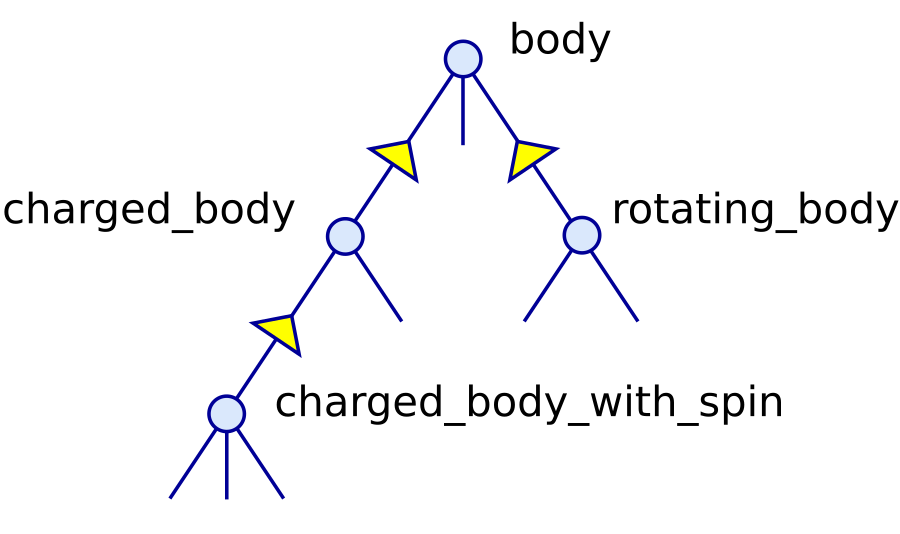
\includegraphics[width=3in,height=\textheight,keepaspectratio]{./images/Inheritance_diagram.png}
\caption{~}
\end{figure}

An object of type \texttt{body} is \textbf{type compatible} with both
\texttt{a\_proton} and \texttt{a\_mutilated\_proton}, so any of these
two can, for example, appear in a call to the procedure \texttt{kick}.

\subsection{Polymorphism}\label{polymorphism}

\subsubsection{\texorpdfstring{Declaring entities with
\texttt{class}}{Declaring entities with class}}\label{declaring-entities-with-class}

By declaring an object with the \texttt{class} instead of the
\texttt{type} specifier, is is possible to defer the actual type that an
object has to be determined when the program executes, or even have the
actual type change during program execution. Such an object is
designated as being \textbf{polymorphic}. To be polymorphic, an object
must fulfill one of the following prerequisites:

\begin{itemize}
\tightlist
\item
  it has the \texttt{pointer} attribute,
\item
  it has the \texttt{allocatable} attribute, or
\item
  it is a dummy argument (with or without a \texttt{pointer} or
  \texttt{allocatable} attribute).
\end{itemize}

For example, the typed alllocation statement executed on a polymorphic
allocatable object

\begin{Shaded}
\begin{Highlighting}[]
\DataTypeTok{class(body)}\NormalTok{, }\DataTypeTok{allocatable} \DataTypeTok{::}\NormalTok{ a\_polymorphic\_body}
\NormalTok{:}
\KeywordTok{allocate}\NormalTok{( charged\_body }\DataTypeTok{::}\NormalTok{ a\_polymorphic\_body )}
\end{Highlighting}
\end{Shaded}

causes the object \texttt{a\_polymorphic\_body} that has the
\textbf{declared} type \texttt{body} to be allocated with the
\textbf{dynamic} type \texttt{charged\_body}; in Fortran nomenclature,
the latter term denotes what was referred to above as ``actual'' type.

\emph{Hint:} For an unallocated allocatable or a disassociated pointer
the dynamic type is considered to be the same as the declared type,
although this is only useful in very few contexts that do not require
the object to be allocated or associated.

\subsubsection{Run-time type and class
identification}\label{run-time-type-and-class-identification}

Within the scope of the object's declaration, only the components of its
declared type are accessible. Also, I/O operations on a polymorphic
object are not permitted, unless UDDTIO routines have been defined. One
way to obtain access to the complete object is to use a construct that
permits \textbf{run-time type identification} (not a Fortran term),
\texttt{select\ type}. For example, the I/O statements in

\begin{Shaded}
\begin{Highlighting}[]
\KeywordTok{select type}\NormalTok{ (a\_polymorphic\_body)}
\KeywordTok{type is}\NormalTok{ (body)}
   \FunctionTok{write(*}\NormalTok{,}\FunctionTok{*)} \StringTok{\textquotesingle{}object of type body has value        \textquotesingle{}}\NormalTok{, a\_polymorphic\_body}
\KeywordTok{type is}\NormalTok{ (charged\_body)}
   \FunctionTok{write(*}\NormalTok{,}\FunctionTok{*)} \StringTok{\textquotesingle{}object of type charged\_body has value\textquotesingle{}}\NormalTok{, a\_polymorphic\_body}
\KeywordTok{class default}
\NormalTok{   error }\KeywordTok{stop} \StringTok{\textquotesingle{}type extension unsupported in this construct\textquotesingle{}}
\KeywordTok{end select}
\end{Highlighting}
\end{Shaded}

are permitted, since inside the block for each \textbf{type guard} the
object is non-polymorphic and of the specified type. At most one type
guard can match the object's type, and the corresponding statements are
executed; otherwise the \texttt{class\ default} section is executed (and
the object remains polymorphic there). A disadvantage of using
\texttt{select\ type} is that it needs to be appropriately updated
whenever an additional type extension is defined; apart from the
maintenance effort this also requires access to all source code that
contain a relevant instance of the construct. For this reason,
type-bound procedures (to be discussed) should be preferably used to
gain access to additional type components.

For updates of the \texttt{charge} component of a \texttt{charged\_body}
object, one now could consider the following:

\begin{Shaded}
\begin{Highlighting}[]
\KeywordTok{subroutine}\NormalTok{ recharge(a\_charged\_body, dq)}
  \DataTypeTok{type(charged\_body)}\NormalTok{, }\DataTypeTok{intent(inout)} \DataTypeTok{::}\NormalTok{ a\_charged\_body}
  \DataTypeTok{real}\NormalTok{, }\DataTypeTok{intent(in)} \DataTypeTok{::}\NormalTok{ dq}

\NormalTok{  a\_charged\_body}\OperatorTok{\%}\NormalTok{charge }\KeywordTok{=}\NormalTok{ a\_charged\_body}\OperatorTok{\%}\NormalTok{charge }\KeywordTok{+}\NormalTok{ dq}
\KeywordTok{end subroutine}
\end{Highlighting}
\end{Shaded}

However, invoking this subroutine in the usual Fortran 95 style will not
work for the variable \texttt{a\_polymorphic\_body}, since it violates
the rule that the dummy argument's declared type must be type compatible
with the actual argument's declared type. One can work around this by
using a \texttt{select\ type} construct with \textbf{run-time class
identification} (not a Fortran term), based on writing \textbf{class
guards} instead of type guards:

\begin{Shaded}
\begin{Highlighting}[]
\KeywordTok{select type}\NormalTok{ (a\_polymorphic\_body)}
\KeywordTok{class is}\NormalTok{ (charged\_body)  }\CommentTok{! new declared type for a\_polymorphic\_body}
  \KeywordTok{call}\NormalTok{ recharge(a\_polymorphic\_body, dq}\KeywordTok{=}\FloatTok{1.0e{-}5}\NormalTok{)}
\KeywordTok{class default}
  \FunctionTok{write(*}\NormalTok{,}\FunctionTok{*)} \StringTok{\textquotesingle{}info: object a\_polymorphic\_body was not modified.\textquotesingle{}}
\KeywordTok{end select}
\end{Highlighting}
\end{Shaded}

The \texttt{recharge} procedure will then be invoked if the dynamic type
of \texttt{a\_polymorphic\_body} is \texttt{charged\_body} or an
extension of it. The object remains polymorphic inside the class guard,
only its declared type changes to that specified in the guard. Unless
the ``lifted'' declared type of interest is already otherwise known from
the context, or handling the \texttt{class\ default} fall-through is
straightforward, this is not in general a desirable way of dealing with
class mismatches.

\emph{Hint:} It is permitted to mix type and class guards in a
\texttt{select\ type} construct; in that case, a type guard has
precedence over a class guard specifying the same type with respect to
selection of the guarded statements to be executed.

\subsubsection{Unlimited polymorphic
objects}\label{unlimited-polymorphic-objects}

A special case of polymorphism is that an object can be
\textbf{unlimited polymorphic}. Such an object, declared with
\texttt{class(*)}, can be of any dynamic type (intrinsic type,
extensible derived type, \texttt{sequence} or \texttt{bind(c)} derived
type), as illustrated by the following statements:

\begin{Shaded}
\begin{Highlighting}[]
\DataTypeTok{class(*)}\NormalTok{, }\DataTypeTok{allocatable} \DataTypeTok{::}\NormalTok{ a\_unlimited  }\CommentTok{! has no declared type, so any type is an extension}

\KeywordTok{allocate}\NormalTok{( a\_unlimited, source}\KeywordTok{=}\FloatTok{2.5e4}\NormalTok{)  }\CommentTok{! dynamic type becomes real}

\KeywordTok{select type}\NormalTok{ ( a\_unlimited )}
\KeywordTok{type is}\NormalTok{ (}\DataTypeTok{real}\NormalTok{)}
  \FunctionTok{write(*}\NormalTok{,}\FunctionTok{*)} \StringTok{\textquotesingle{}a\_unlimited is of intrinsic real type with value \textquotesingle{}}\NormalTok{, a\_unlimited}
\KeywordTok{end select}

\KeywordTok{deallocate}\NormalTok{( a\_unlimited )}
\KeywordTok{allocate}\NormalTok{( a\_unlimited, source}\KeywordTok{=}\NormalTok{a\_proton) )  }\CommentTok{! dynamic type becomes charged\_body}

\KeywordTok{select type}\NormalTok{ ( a\_unlimited )}
\KeywordTok{type is}\NormalTok{ (charged\_body)}
  \FunctionTok{write(*}\NormalTok{,}\FunctionTok{*)} \StringTok{\textquotesingle{}a\_unlimited is a charged\_body with value \textquotesingle{}}\NormalTok{, a\_unlimited}
\KeywordTok{end select}
\end{Highlighting}
\end{Shaded}

Accessing the object's data \emph{always} needs a \texttt{select\ type}
construct; type guards in the construct can in this case might not only
refer to extensible types, but also to intrinsic types. However, for
\texttt{sequence} or \texttt{bind(c)} derived types, no type resolution
is possible - these always fall through to a \texttt{class\ default}
guard, if present; use of unlimited polymorphic objects to store values
of such types is therefore considered unsafe.

In this context, allocation with \texttt{source=} allocates the target
object to the source object's dynamic type before copying its value to
the target object. If the source object's data is not needed,
\texttt{mold=} can be used instead. Sourced allocation becomes a
powerful tool, since the dynamic type of the source object need not be
known in the scoping unit within which the allocation is executed.

Type components with the \texttt{pointer} or \texttt{allocatable}
attribute can be unlimited polymorphic, enabling the construction of
generic and potentially inhomogeneous container-like types. As an
illustration of this, a supporting type for the purpose of holding data
targeted for manipulation of other objects is presented; its definition
(placed in the module \texttt{mod\_utility\_types}) reads

\begin{Shaded}
\begin{Highlighting}[]
\DataTypeTok{type} \DataTypeTok{::}\NormalTok{ any\_object}
  \DataTypeTok{character(len=:)}\NormalTok{, }\DataTypeTok{allocatable} \DataTypeTok{::}\NormalTok{ description}
  \DataTypeTok{class(*)}\NormalTok{, }\DataTypeTok{allocatable} \DataTypeTok{::} \DataTypeTok{value}\NormalTok{(:)}
  \DataTypeTok{integer}\NormalTok{, }\DataTypeTok{allocatable} \DataTypeTok{::} \FunctionTok{shape}\NormalTok{(:)}
\DataTypeTok{end type}
\end{Highlighting}
\end{Shaded}

where \texttt{description} will refer to the property that needs
updating, and \texttt{value} will contain the data to be used for the
transaction. Because the \texttt{value} component should be able to
represent any type, it is declared as being unlimited polymorphic.
Because the \texttt{value} component might hold data needed to produce
an array of arbitrary shape, the additional \texttt{shape} component is
supplied, but its use is really only necessary if objects of rank at
least 2 must be dealt with. The structure constructor for that type has
been overloaded to work around compiler bugs and make handling of scalar
data easier. The following example illustrates how to establish a simple
interface for setting components of a structure:

\begin{Shaded}
\begin{Highlighting}[]
\KeywordTok{module}\NormalTok{ mod\_wtype}
  \KeywordTok{use}\NormalTok{ mod\_utility\_types, }\KeywordTok{only}\NormalTok{ : initialize }\KeywordTok{=}\OperatorTok{\textgreater{}}\NormalTok{ any\_object}

  \DataTypeTok{type} \DataTypeTok{::}\NormalTok{ wtype}
    \DataTypeTok{private}
    \DataTypeTok{integer} \DataTypeTok{::}\NormalTok{ nonzeros }\KeywordTok{=} \KeywordTok{{-}}\DecValTok{1}
    \DataTypeTok{real}\NormalTok{, }\DataTypeTok{allocatable} \DataTypeTok{::}\NormalTok{ w(:,:)}
  \DataTypeTok{end type}\NormalTok{ wtype}
\KeywordTok{contains}
  \KeywordTok{subroutine}\NormalTok{ setup\_wtype(a\_wtype, a\_component)}
    \CommentTok{! in{-}place setting to avoid memory bursts for large objects}
    \DataTypeTok{type(wtype)}\NormalTok{, }\DataTypeTok{intent(inout)} \DataTypeTok{::}\NormalTok{ a\_wtype}
    \DataTypeTok{type(initialize)}\NormalTok{, }\DataTypeTok{intent(in)}\NormalTok{, }\DataTypeTok{target} \DataTypeTok{::}\NormalTok{ a\_component}
    \DataTypeTok{integer} \DataTypeTok{::}\NormalTok{ wsize}
    \DataTypeTok{real}\NormalTok{, }\DataTypeTok{pointer} \DataTypeTok{::}\NormalTok{ pw(:,:)}

    \KeywordTok{select case}\NormalTok{ (a\_component}\OperatorTok{\%}\NormalTok{description)}
     \KeywordTok{case}\NormalTok{ (}\StringTok{"nonzeros"}\NormalTok{)}
      \KeywordTok{if}\NormalTok{ ( }\FunctionTok{allocated}\NormalTok{(a\_component}\OperatorTok{\%}\DataTypeTok{value}\NormalTok{) ) }\KeywordTok{then}
        \KeywordTok{select type}\NormalTok{ ( nonzeros }\KeywordTok{=}\OperatorTok{\textgreater{}}\NormalTok{ a\_component}\OperatorTok{\%}\DataTypeTok{value}\NormalTok{(}\DecValTok{1}\NormalTok{) )}
         \KeywordTok{type is}\NormalTok{ (}\DataTypeTok{integer}\NormalTok{)}
\NormalTok{          a\_wtype}\OperatorTok{\%}\NormalTok{nonzeros }\KeywordTok{=}\NormalTok{ nonzeros}
        \KeywordTok{end select}
      \KeywordTok{end if}
     \KeywordTok{case}\NormalTok{ (}\StringTok{"w"}\NormalTok{)}
      \KeywordTok{if}\NormalTok{ ( }\FunctionTok{allocated}\NormalTok{(a\_component}\OperatorTok{\%}\DataTypeTok{value}\NormalTok{) }\OperatorTok{.and.} \FunctionTok{allocated}\NormalTok{(a\_component}\OperatorTok{\%}\FunctionTok{shape}\NormalTok{) ) }\KeywordTok{then}
\NormalTok{        wsize }\KeywordTok{=} \FunctionTok{size}\NormalTok{(a\_component}\OperatorTok{\%}\DataTypeTok{value}\NormalTok{)}
        \KeywordTok{if}\NormalTok{ ( wsize }\OperatorTok{\textgreater{}=} \FunctionTok{product}\NormalTok{(a\_component}\OperatorTok{\%}\FunctionTok{shape}\NormalTok{) ) }\KeywordTok{then}
          \KeywordTok{select type}\NormalTok{ ( w }\KeywordTok{=}\OperatorTok{\textgreater{}}\NormalTok{ a\_component}\OperatorTok{\%}\DataTypeTok{value}\NormalTok{ )}
           \KeywordTok{type is}\NormalTok{ (}\DataTypeTok{real}\NormalTok{)}
\NormalTok{            pw(}\DecValTok{1}\NormalTok{:a\_component}\OperatorTok{\%}\FunctionTok{shape}\NormalTok{(}\DecValTok{1}\NormalTok{), }\DecValTok{1}\NormalTok{:a\_component}\OperatorTok{\%}\FunctionTok{shape}\NormalTok{(}\DecValTok{2}\NormalTok{)) }\KeywordTok{=}\OperatorTok{\textgreater{}}\NormalTok{ w}
\NormalTok{            a\_wtype}\OperatorTok{\%}\NormalTok{w }\KeywordTok{=}\NormalTok{ pw}
          \KeywordTok{end select}
        \KeywordTok{end if}
      \KeywordTok{end if}
    \KeywordTok{end select}
  \KeywordTok{end subroutine}\NormalTok{ setup\_wtype}
\NormalTok{  :}
\KeywordTok{end module}
\end{Highlighting}
\end{Shaded}

\textbf{Notes:}

\begin{itemize}
\tightlist
\item
  Having this simple interface at the cost of significant additional
  setup code might at first sight appear frivolous; however, once type
  extension is used on a larger scale, setting or modifying further
  components in the conventional way becomes rather irksome without a
  concept like that above, especially if \hyperref[sec:tbp]{type-bound
  procedures} with a simple \emph{and} uniform interface must be
  implemented;
\item
  The object \texttt{a\_wtype} remains unchanged in case an unsuitable
  value is provided for \texttt{a\_component}. One could add explicit
  error handling, but for these examples this is considered an
  unnecessary complication;
\item
  The permitted values for the \texttt{initialize} object should be
  documented for each procedure that takes such an object;
\item
  Because access to \texttt{a\_component} within \texttt{select\ type}
  is via a type component, one is obliged to introduce an associate name
  for the latter. The language rules only permit omitting the associate
  name for named variables, and subobjects are not named variables;
\item
  A \textbf{rank-changing pointer assignment} is used to transform the
  rank-1 \texttt{a\_component\%value} array to an object that can be
  assigned to a rank-2 \texttt{a\_wtype\%w} array; this works because
  the right-hand side is a rank-1 object; for rank-2 and higher the
  rank-changing pointer assignment will only work if the target assigned
  to is a \textbf{simply contiguous array designator} (a topic not
  covered here). Note that in this context, the \texttt{reshape}
  intrinsic cannot be used because it requires the size of its
  \texttt{shape} argument to be a constant.
\end{itemize}

The program invoking the \texttt{setup\_wtype} procedure might do so as
follows, to set up a \texttt{wtype} object:

\begin{Shaded}
\begin{Highlighting}[]
\KeywordTok{use}\NormalTok{ mod\_wtype}
\DataTypeTok{type(initialize)} \DataTypeTok{::}\NormalTok{ c\_nz, c\_w}
\DataTypeTok{type(wtype)} \DataTypeTok{::}\NormalTok{ my\_wtype}
\DataTypeTok{integer} \DataTypeTok{::}\NormalTok{ i, j}
\DataTypeTok{integer} \DataTypeTok{::}\NormalTok{ ndim}

\NormalTok{ndim }\KeywordTok{=}\NormalTok{ ...}

\KeywordTok{associate}\NormalTok{ ( my\_data }\KeywordTok{=}\OperatorTok{\textgreater{}} \KeywordTok{[}\NormalTok{ ((}\DataTypeTok{real (max(0, min(i{-}j+2, j{-}i+2)))}\NormalTok{, j}\KeywordTok{=}\DecValTok{1}\NormalTok{, ndim), i}\KeywordTok{=}\DecValTok{1}\NormalTok{, ndim) }\KeywordTok{]}\NormalTok{ )}
\NormalTok{  c\_nz }\KeywordTok{=}\NormalTok{ initialize(}\StringTok{"nonzeros"}\NormalTok{, }\FunctionTok{count}\NormalTok{(my\_data }\OperatorTok{/=} \DecValTok{0}\NormalTok{))}
\NormalTok{  c\_w }\KeywordTok{=}\NormalTok{ initialize(}\StringTok{"w"}\NormalTok{, my\_data, }\KeywordTok{[}\NormalTok{ ndim, ndim }\KeywordTok{]}\NormalTok{ )}
\KeywordTok{end associate}

\KeywordTok{call}\NormalTok{ setup\_wtype(my\_wtype, c\_nz)}
\KeywordTok{call}\NormalTok{ setup\_wtype(my\_wtype, c\_w)}
\end{Highlighting}
\end{Shaded}

\subsection{Type-bound procedures (TBP)}\label{sec:tbp}

To resolve the class mismatch issues arising from the use of polymorphic
objects, one needs a language mechanism for making a run-time decision
on a procedure invocation that depends on the dynamic type of a
polymorphic object. This can be achieved by binding a procedure to a
type in the type definition via a \texttt{procedure} statement in the
type's \texttt{contains} part.

For the type \texttt{body}, the augmented type definition reads

\begin{Shaded}
\begin{Highlighting}[]
\DataTypeTok{type} \DataTypeTok{::}\NormalTok{ body}
  \DataTypeTok{real} \DataTypeTok{::}\NormalTok{ mass}
  \DataTypeTok{real} \DataTypeTok{::}\NormalTok{ pos(}\DecValTok{3}\NormalTok{), vel(}\DecValTok{3}\NormalTok{)}
\KeywordTok{contains}
  \DataTypeTok{procedure} \DataTypeTok{::}\NormalTok{ update }\KeywordTok{=}\OperatorTok{\textgreater{}}\NormalTok{ update\_body}
\DataTypeTok{end type}
\end{Highlighting}
\end{Shaded}

This does not impact how the structure constructor is used; for this,
only the specifications before the \texttt{contains} statement are
relevant. To establish a simple and uniform interface for object
updates, the procedure \texttt{update\_body} makes use of the
\texttt{any\_object} type discussed earlier, which in view of the
context is locally renamed to \texttt{change}:

\begin{Shaded}
\begin{Highlighting}[]
\KeywordTok{subroutine}\NormalTok{ update\_body(a\_body, a\_change)}
  \DataTypeTok{class(body)}\NormalTok{, }\DataTypeTok{intent(inout)} \DataTypeTok{::}\NormalTok{ a\_body}
  \DataTypeTok{type(change)}\NormalTok{, }\DataTypeTok{intent(in)} \DataTypeTok{::}\NormalTok{ a\_change}
  \KeywordTok{if}\NormalTok{ ( }\FunctionTok{allocated}\NormalTok{(a\_change}\OperatorTok{\%}\NormalTok{description) }\OperatorTok{.and.} \FunctionTok{allocated}\NormalTok{(a\_change}\OperatorTok{\%}\DataTypeTok{value}\NormalTok{) ) }\KeywordTok{then}
    \KeywordTok{select case}\NormalTok{ ( }\FunctionTok{trim}\NormalTok{(a\_change}\OperatorTok{\%}\NormalTok{description) )}
     \KeywordTok{case}\NormalTok{ (}\StringTok{\textquotesingle{}mass\textquotesingle{}}\NormalTok{)}
      \KeywordTok{select type}\NormalTok{ ( delta }\KeywordTok{=}\OperatorTok{\textgreater{}}\NormalTok{ a\_change}\OperatorTok{\%}\DataTypeTok{value}\NormalTok{(}\DecValTok{1}\NormalTok{) )}
       \KeywordTok{type is}\NormalTok{ (}\DataTypeTok{real}\NormalTok{)}
        \KeywordTok{call}\NormalTok{ accrete(a\_body, delta)}
      \KeywordTok{end select}
     \KeywordTok{case}\NormalTok{ (}\StringTok{\textquotesingle{}momentum\textquotesingle{}}\NormalTok{)}
      \KeywordTok{select type}\NormalTok{ ( delta }\KeywordTok{=}\OperatorTok{\textgreater{}}\NormalTok{ a\_change}\OperatorTok{\%}\DataTypeTok{value}\NormalTok{ )}
       \KeywordTok{type is}\NormalTok{ (}\DataTypeTok{real}\NormalTok{)}
        \KeywordTok{if}\NormalTok{ ( }\FunctionTok{size}\NormalTok{(delta) }\OperatorTok{\textgreater{}=} \DecValTok{3}\NormalTok{ ) }\KeywordTok{call}\NormalTok{ kick(a\_body, delta(}\DecValTok{1}\NormalTok{:}\DecValTok{3}\NormalTok{))}
      \KeywordTok{end select}
     \KeywordTok{case}\NormalTok{ (}\StringTok{\textquotesingle{}position\textquotesingle{}}\NormalTok{)}
      \KeywordTok{select type}\NormalTok{ ( delta }\KeywordTok{=}\OperatorTok{\textgreater{}}\NormalTok{ a\_change}\OperatorTok{\%}\DataTypeTok{value}\NormalTok{ )}
       \KeywordTok{type is}\NormalTok{ (}\DataTypeTok{real}\NormalTok{)}
        \KeywordTok{if}\NormalTok{ ( }\FunctionTok{size}\NormalTok{(delta) }\OperatorTok{\textgreater{}=} \DecValTok{3}\NormalTok{) a\_body}\OperatorTok{\%}\NormalTok{pos }\KeywordTok{=}\NormalTok{ a\_body}\OperatorTok{\%}\NormalTok{pos }\KeywordTok{+}\NormalTok{ delta(}\DecValTok{1}\NormalTok{:}\DecValTok{3}\NormalTok{)}
      \KeywordTok{end select}
    \KeywordTok{end select}
  \KeywordTok{end if}
\KeywordTok{end subroutine}
\end{Highlighting}
\end{Shaded}

In its interface, the \textbf{passed object} \texttt{a\_body} must be
declared to be a polymorphic scalar, with its declared type being the
one the procedure has been bound to. The implementation reuses existing
code where possible (very simple in this example, but this is of course
not generally the case), to avoid the need for extensive revalidation.

Invocation of the procedure could be done in the usual manner, but the
preferred style, especially in the case that the actual argument is
polymorphic, is to do it through the object itself:

\begin{Shaded}
\begin{Highlighting}[]
\DataTypeTok{Type(change)} \DataTypeTok{::}\NormalTok{  dx}
\NormalTok{:}
\NormalTok{dx }\KeywordTok{=}\NormalTok{ change(description}\KeywordTok{=}\StringTok{\textquotesingle{}mass\textquotesingle{}}\NormalTok{, }\DataTypeTok{value}\KeywordTok{=[}\FloatTok{0.0}\NormalTok{, }\FloatTok{2.0}\NormalTok{, }\FloatTok{0.0}\KeywordTok{]}\NormalTok{)}

\KeywordTok{call}\NormalTok{ my\_basketball}\OperatorTok{\%}\NormalTok{update(dx) }\CommentTok{! invokes update\_body(my\_basketball, dx)}
\end{Highlighting}
\end{Shaded}

For polymorphic objects, the procedure \texttt{update\_body} will be
invoked if the dynamic type of the object is \texttt{body} (this might
not be true if the dynamic type is an extension, as we shall see).

\emph{Hint:} The invocation can also be done with non-polymorphic
objects; in this case, the binding could (in principle) be determined at
compilation time, potentially saving some call overhead. Note that the
passed object dummy is not permitted to be allocatable or a pointer,
which facilitates this usage.

So far this is not particularly interesting; the key thing is what
happens once we turn to type extensions. For example, to enable
modification of the \texttt{charge} component (in addition to that of
other components) of an object of dynamic type \texttt{charged\_body},
it is possible to \textbf{override} the parent type's bound procedure:

\begin{Shaded}
\begin{Highlighting}[]
\DataTypeTok{type}\NormalTok{, }\DataTypeTok{extends(body)} \DataTypeTok{::}\NormalTok{ charged\_body}
  \DataTypeTok{real} \DataTypeTok{::}\NormalTok{ charge}
\KeywordTok{contains}
  \DataTypeTok{procedure} \DataTypeTok{::}\NormalTok{ update }\KeywordTok{=}\OperatorTok{\textgreater{}}\NormalTok{ update\_charged\_body}
\DataTypeTok{end type}
\end{Highlighting}
\end{Shaded}

with the procedure defined as follows:

\begin{Shaded}
\begin{Highlighting}[]
\KeywordTok{subroutine}\NormalTok{ update\_charged\_body(a\_body, a\_change)}
  \DataTypeTok{class(charged\_body)} \DataTypeTok{::}\NormalTok{ a\_body}
  \DataTypeTok{type(change)} \DataTypeTok{::}\NormalTok{ a\_change}

  \KeywordTok{if}\NormalTok{ ( }\FunctionTok{allocated}\NormalTok{(a\_change}\OperatorTok{\%}\NormalTok{description) }\OperatorTok{.and.} \FunctionTok{allocated}\NormalTok{(a\_change}\OperatorTok{\%}\DataTypeTok{value}\NormalTok{) ) }\KeywordTok{then}
    \KeywordTok{select case}\NormalTok{ ( }\FunctionTok{trim}\NormalTok{(a\_change}\OperatorTok{\%}\NormalTok{description) )}
     \KeywordTok{case}\NormalTok{ (}\StringTok{\textquotesingle{}charge\textquotesingle{}}\NormalTok{)}
      \KeywordTok{select type}\NormalTok{ ( delta }\KeywordTok{=}\OperatorTok{\textgreater{}}\NormalTok{ a\_change}\OperatorTok{\%}\DataTypeTok{value}\NormalTok{(}\DecValTok{1}\NormalTok{) )}
       \KeywordTok{type is}\NormalTok{ (}\DataTypeTok{real}\NormalTok{)}
\NormalTok{        a\_body}\OperatorTok{\%}\NormalTok{charge }\KeywordTok{=}\NormalTok{ a\_body}\OperatorTok{\%}\NormalTok{charge }\KeywordTok{+}\NormalTok{ delta}
      \KeywordTok{end select}
     \KeywordTok{case default}
      \KeywordTok{call}\NormalTok{ a\_body}\OperatorTok{\%}\NormalTok{body}\OperatorTok{\%}\NormalTok{update(a\_change)}
      \CommentTok{! assure that a change to a parent component is dealt with}
    \KeywordTok{end select}
  \KeywordTok{end if}
\KeywordTok{end subroutine}
\end{Highlighting}
\end{Shaded}

The overriding procedure must use the same interface as the overridden
procedure, except that the passed object is declared to be of the
extended type; even the argument keywords must be the same. Once the
override has been defined, the call through an object of dynamic type
\texttt{charged\_body} will be dispatched to
\texttt{update\_charged\_body}:

\begin{Shaded}
\begin{Highlighting}[]
\DataTypeTok{type(change)} \DataTypeTok{::}\NormalTok{  dc, dp}
\DataTypeTok{class(body)}\NormalTok{, }\DataTypeTok{allocatable} \DataTypeTok{::}\NormalTok{ my\_polymorphic\_body}

\NormalTok{my\_polymorphic\_body }\KeywordTok{=}\NormalTok{ charged\_body(mass}\KeywordTok{=}\FloatTok{1.5}\NormalTok{, pos}\KeywordTok{=[}\FloatTok{0.}\NormalTok{,}\FloatTok{0.}\NormalTok{,}\FloatTok{0.}\KeywordTok{]}\NormalTok{, }\KeywordTok{\&}
\NormalTok{                                   vel}\KeywordTok{=[}\FloatTok{2.}\NormalTok{,}\FloatTok{0.}\NormalTok{,}\FloatTok{0.}\KeywordTok{]}\NormalTok{, charge}\KeywordTok{=}\FloatTok{2.41e{-}5}\NormalTok{)}
\CommentTok{! the above statement auto{-}allocates the left hand side}
\NormalTok{dc }\KeywordTok{=}\NormalTok{ change(description}\KeywordTok{=}\StringTok{\textquotesingle{}charge\textquotesingle{}}\NormalTok{, }\DataTypeTok{value}\KeywordTok{=}\FloatTok{5.0e{-}6}\NormalTok{)}
\NormalTok{dp }\KeywordTok{=}\NormalTok{ change(description}\KeywordTok{=}\StringTok{\textquotesingle{}momentum\textquotesingle{}}\NormalTok{, }\DataTypeTok{value}\KeywordTok{=[{-}}\FloatTok{1.0}\NormalTok{,}\FloatTok{1.0}\NormalTok{,}\FloatTok{0.0}\KeywordTok{]}\NormalTok{)}

\CommentTok{! both the following dispatch to update\_charged\_body}
\KeywordTok{call}\NormalTok{ my\_polymorphic\_body}\OperatorTok{\%}\NormalTok{update(dc)}
\KeywordTok{call}\NormalTok{ my\_polymorphic\_body}\OperatorTok{\%}\NormalTok{update(dp)}
\end{Highlighting}
\end{Shaded}

\textbf{Notes:}

\begin{itemize}
\tightlist
\item
  for the above example, direct invocation of the procedure
  \texttt{update\_charged\_body} is not possible (as already noted
  earlier);
\item
  the second TBP call illustrates the invocation of the parent object
  update from \texttt{update\_charged\_body}. Without this, changes that
  impact the parent object would not be done. By implementing this
  consistency of behaviour, the programmer assures that the inheritance
  hierarchy adheres to the
  \href{https://en.wikipedia.org/wiki/Liskov_substitution_principle}{Liskov
  substitution principle};
\item
  to enforce using the TBP calls in a use association context, the
  module procedures that implement them can be made \texttt{private}.
  The accessibility of the TBP itself is determined by the attribute for
  it (default is \texttt{public}) in the type definition;
\item
  the programmer can prevent overriding of a binding by declaring it to
  be \texttt{non\_overridable}; its implementation then is regarded as
  valid for all conceivable extension types.
\end{itemize}

\subsection{Abstract types and
interfaces}\label{abstract-types-and-interfaces}

The \texttt{sortable} type used for demonstrating the
\texttt{sortable\_list} functionality in the
\hyperref[sec:oop_techniques]{object-based chapter's} example was set up
as a fixed container-like type. It is desirable to be able to use the
list machinery more flexibly i.e., for any type that supports the
``less-than'' comparison. This can be achieved by introducing an
\textbf{abstract type}

\begin{Shaded}
\begin{Highlighting}[]
\DataTypeTok{type}\NormalTok{, }\DataTypeTok{abstract} \DataTypeTok{::}\NormalTok{ sortable}
\KeywordTok{contains}
  \DataTypeTok{procedure(compare)}\NormalTok{, }\DataTypeTok{deferred} \DataTypeTok{::}\NormalTok{ less\_than}
  \CommentTok{! ... more to follow}
\DataTypeTok{end type}
\end{Highlighting}
\end{Shaded}

with a \textbf{deferred binding}. It is not possible to create an object
whose dynamic type is abstract, or a non-polymorphic object of abstract
type. For this reason, the deferred binding cannot represent an existing
procedure, but is characterized by an \textbf{abstract interface}:

\begin{Shaded}
\begin{Highlighting}[]
\DataTypeTok{abstract} \KeywordTok{interface}
  \KeywordTok{pure} \DataTypeTok{logical} \KeywordTok{function}\NormalTok{ compare(s1, s2)}
    \KeywordTok{import} \DataTypeTok{::}\NormalTok{ sortable}
    \DataTypeTok{class(sortable)}\NormalTok{, }\DataTypeTok{intent(in)} \DataTypeTok{::}\NormalTok{ s1, s2}
    \CommentTok{! dispatch is via the first argument}
  \KeywordTok{end function}
\KeywordTok{end interface}
\end{Highlighting}
\end{Shaded}

The \texttt{import} statement is required to give the interface access
to the type defined in its host. Furthermore, an override of the
structure constructor will be needed

\begin{Shaded}
\begin{Highlighting}[]
\KeywordTok{interface}\NormalTok{ sortable}
  \DataTypeTok{procedure} \DataTypeTok{::}\NormalTok{ create\_sortable}
\KeywordTok{end interface}
\end{Highlighting}
\end{Shaded}

that permits creation of polymorphic \texttt{sortable} objects. The
details of this will be described later (since, indeed, a devil lurks in
these details). Note that the above combined use of abstract types and
interfaces is also known under the (non-Fortran) term \textbf{interface
class}.

This framework permits the programmer to implement the following
programming technique, which is also known as \textbf{dependency
inversion} (not a Fortran term):

\begin{enumerate}
\def\labelenumi{\arabic{enumi}.}
\item
  Any machinery that makes use of polymorphic \texttt{sortable} objects
  is made to only refer to the above abstractions. For example, the
  definition of the \texttt{sorted\_list} type could be adapted to read

\begin{Shaded}
\begin{Highlighting}[]
\DataTypeTok{type}\NormalTok{, }\DataTypeTok{public} \DataTypeTok{::}\NormalTok{ sorted\_list}
  \DataTypeTok{private}
  \DataTypeTok{class(sortable)}\NormalTok{, }\DataTypeTok{allocatable} \DataTypeTok{::}\NormalTok{ data}
  \CommentTok{! changed to refer to abstract type}
  \DataTypeTok{type(sorted\_list)}\NormalTok{, }\DataTypeTok{pointer} \DataTypeTok{::}\NormalTok{ next }\KeywordTok{=}\OperatorTok{\textgreater{}}\NormalTok{ null()}
\KeywordTok{contains}
  \DataTypeTok{final} \DataTypeTok{::}\NormalTok{ delete\_sorted\_list}
\DataTypeTok{end type}
\end{Highlighting}
\end{Shaded}

  The advantage of this is that no change to the preexisting machinery
  will be needed whenever a programmer decides to add an extension type
  as outlined in 2. below.
\item
  For a concrete realization of a \texttt{sortable} object, the
  programmer needs to create a type extension, for example

\begin{Shaded}
\begin{Highlighting}[]
\DataTypeTok{type}\NormalTok{, }\DataTypeTok{public}\NormalTok{, }\DataTypeTok{extends(sortable)} \DataTypeTok{::}\NormalTok{ sortable\_string}
  \DataTypeTok{character(len=:)}\NormalTok{, }\DataTypeTok{allocatable} \DataTypeTok{::}\NormalTok{ string}
\KeywordTok{contains}
  \DataTypeTok{procedure} \DataTypeTok{::}\NormalTok{ less\_than }\KeywordTok{=}\OperatorTok{\textgreater{}}\NormalTok{ less\_than\_string}
\DataTypeTok{end type}
\end{Highlighting}
\end{Shaded}

  including an \emph{obligatory} implementation
  \texttt{less\_than\_string} of an overriding TBP for the deferred
  binding. The constructor function (promised earlier, but not yet
  delivered) also needs to be updated to enable creation of objects of
  the extended type.
\end{enumerate}

\subsection{Generic type-bound procedures and operator
overloading}\label{generic-type-bound-procedures-and-operator-overloading}

As a convenience, use of an overloading for the comparison operator
``\textless{}'' can be provided by creating a \textbf{generic}
type-bound procedure:

\begin{Shaded}
\begin{Highlighting}[]
\DataTypeTok{type}\NormalTok{, }\DataTypeTok{abstract} \DataTypeTok{::}\NormalTok{ sortable}
\KeywordTok{contains}
  \DataTypeTok{procedure(compare)}\NormalTok{, }\DataTypeTok{deferred} \DataTypeTok{::}\NormalTok{ less\_than}
  \DataTypeTok{generic} \DataTypeTok{::} \KeywordTok{operator}\NormalTok{(}\OperatorTok{\textless{}}\NormalTok{) }\KeywordTok{=}\OperatorTok{\textgreater{}}\NormalTok{ less\_than}
\DataTypeTok{end type}
\end{Highlighting}
\end{Shaded}

which means that when a statement involving a comparison expression

\begin{Shaded}
\begin{Highlighting}[]
\DataTypeTok{class(sortable)}\NormalTok{, }\DataTypeTok{allocatable} \DataTypeTok{::}\NormalTok{ s1, s2}

\NormalTok{s1 }\KeywordTok{=}\NormalTok{ sortable( ... )}
\NormalTok{s2 }\KeywordTok{=}\NormalTok{ sortable( ... )}

\KeywordTok{if}\NormalTok{ ( s1 }\OperatorTok{\textless{}}\NormalTok{ s2 ) }\KeywordTok{then}
\NormalTok{   ...}
\KeywordTok{end if}
\end{Highlighting}
\end{Shaded}

is executed, the overridden type-bound procedure bound to the first
operand will be invoked to evaluate the expression. It is not necessary
to re-specify the \texttt{generic} clause in any type extensions; the
dispatch will automatically select the overridden procedure.

Named generic type-bound procedures that do not overload existing
operations can also be defined; an example for this is given in the
section ``\hyperref[sec:functions_with_parameters]{Functions with
parameters}''. The rules for generic resolution work similar as for
nonpolymorphic generic procedure interfaces, with the additional
restriction that polymorphic dummy arguments that are related by
inheritance cannot be distinguished for the purpose of compile-time
resolution to a specific procedure.

\subsection{Completing the dependency
inversion}\label{completing-the-dependency-inversion}

\subsubsection{Discussion of structural
dependencies}\label{discussion-of-structural-dependencies}

When implementing the above concept, typically a separate module, say
\texttt{mod\_sortable\_extensions}, is created for some or all of the
extension types of \texttt{sortable}. The motivations for this can be:

\begin{itemize}
\tightlist
\item
  avoid recompilation of any machinery that makes use of the
  \texttt{mod\_sortable} module;
\item
  the source code of \texttt{mod\_sortable} might not be readily
  modifiable;
\item
  prevent \texttt{mod\_sortable} from turning into a monster module in
  case large concepts are implemented through extension types, or many
  extension types are created.
\end{itemize}

The implementation of the constructor will need to use associate
\texttt{mod\_sortable\_extensions} since it needs to be able to create
objects of the types defined there. On the other hand, the interface to
the constructor needs to be visible in \texttt{mod\_sortable}, since the
machinery that depends on it must be able to call it. As a consequence,
one would end up with a circular \texttt{use} dependency between the two
modules, which is prohibited.

\subsubsection{Using submodules to break dependency
cycles}\label{using-submodules-to-break-dependency-cycles}

To deal with such a situation (among others), the concept of
\textbf{submodule} is available. This is a type of program unit that
serves as an extension to an existing module (or submodule), to which it
has access by host association. Furthermore, submodules allow the
programmer to separate interfaces from implementations; the former are
defined in the parent program unit (i.e., the program unit of which the
submodule is an extension), the latter in the submodule itself.

For the constructor function, the following interface block can be
declared in \texttt{mod\_sortable}:

\begin{Shaded}
\begin{Highlighting}[]
\KeywordTok{interface}
  \KeywordTok{module} \KeywordTok{function}\NormalTok{ create\_sortable(init) }\KeywordTok{result}\NormalTok{(r)}
    \DataTypeTok{class(sortable)}\NormalTok{, }\DataTypeTok{allocatable} \DataTypeTok{::}\NormalTok{ r}
    \DataTypeTok{type(initialize)}\NormalTok{, }\DataTypeTok{intent(in)} \DataTypeTok{::}\NormalTok{ init}
  \KeywordTok{end function}
\KeywordTok{end interface}
\end{Highlighting}
\end{Shaded}

The special notation \texttt{module\ function} (or
\texttt{module\ subroutine} for a subroutine) tells the compiler that
the implementation is deferred to a submodule.

\textbf{Notes:}

\begin{itemize}
\tightlist
\item
  the above interface requires no reference to any entities contained in
  \texttt{mod\_sortable\_extensions};
\item
  consistent with this, the variable representing the function result is
  an allocatable polymorphic object of the abstract type;
\item
  an \texttt{import} statement is not obligatory in separate module
  procedure interfaces, although it is permitted (compiler support
  assumed!), primarily for the purpose of fine-grain control of host
  access;
\item
  the type \texttt{initialize} is, again, a renamed version of the
  \texttt{any\_object} type referred to earlier.
\end{itemize}

\subsubsection{Implementation of the
constructor}\label{implementation-of-the-constructor}

The submodule containing the implementation then reads as follows:

\begin{Shaded}
\begin{Highlighting}[]
\KeywordTok{submodule}\NormalTok{ (mod\_sortable) smod\_constructor}
\KeywordTok{contains}
  \KeywordTok{module procedure}\NormalTok{ create\_sortable}
  \KeywordTok{use}\NormalTok{ mod\_sortable\_extensions, }\KeywordTok{only}\NormalTok{ : sortable\_string}

  \KeywordTok{if}\NormalTok{ ( }\FunctionTok{allocated}\NormalTok{(init}\OperatorTok{\%}\NormalTok{description) }\OperatorTok{.and.} \FunctionTok{allocated}\NormalTok{(init}\OperatorTok{\%}\DataTypeTok{value}\NormalTok{) ) }\KeywordTok{then}
    \KeywordTok{select case}\NormalTok{ (init}\OperatorTok{\%}\NormalTok{description)}
     \KeywordTok{case}\NormalTok{ (}\StringTok{\textquotesingle{}sortable\_string\textquotesingle{}}\NormalTok{)}
      \KeywordTok{select type}\NormalTok{ ( }\DataTypeTok{value} \KeywordTok{=}\OperatorTok{\textgreater{}}\NormalTok{ init}\OperatorTok{\%}\DataTypeTok{value}\NormalTok{(}\DecValTok{1}\NormalTok{) )}
       \KeywordTok{type is}\NormalTok{ (}\DataTypeTok{character(len=*)}\NormalTok{)}
        \KeywordTok{allocate}\NormalTok{( r, source}\KeywordTok{=}\NormalTok{sortable\_string(}\DataTypeTok{value}\NormalTok{) )}
      \KeywordTok{end select}
    \KeywordTok{end select}
  \KeywordTok{end if}
\KeywordTok{end procedure}
\KeywordTok{end submodule}
\end{Highlighting}
\end{Shaded}

\textbf{Notes:}

\begin{itemize}
\tightlist
\item
  The interface for the separate module procedures is omitted, since it
  can be deduced from its specification in the parent module. However,
  alternative syntax exists that replicates the interface (but this is
  not shown here);
\item
  the effect of the \texttt{only} clause is to suppress use access to
  any entity of the parent program unit (which would be indirectly
  established). This is because use association overrides host
  association, which may cause undesirable side effects;
\item
  submodules additionally can contain specifications (before the
  \texttt{contains} statement), as well as local submodule procedures.
  All these are only accessible from the submodule (and its descendant
  submodules, if any);
\item
  the naming scheme for a submodule always references the direct parent.
  For submodules of submodules, the scheme is
  \texttt{submodule\ (\textless{}parent\ module\textgreater{}:\textless{}parent\ submodule\textgreater{})\ \textless{}submodule\_name\textgreater{}}
  and the names of submodules of a given module must be unique.
\end{itemize}

\subsubsection{Diagramming the dependencies between program
units}\label{diagramming-the-dependencies-between-program-units}

The following diagram shows the use and host association relationships
between the modules (blue boxes), the submodule (green box), and a main
program unit (orange box) for this example:

\begin{figure}
\centering
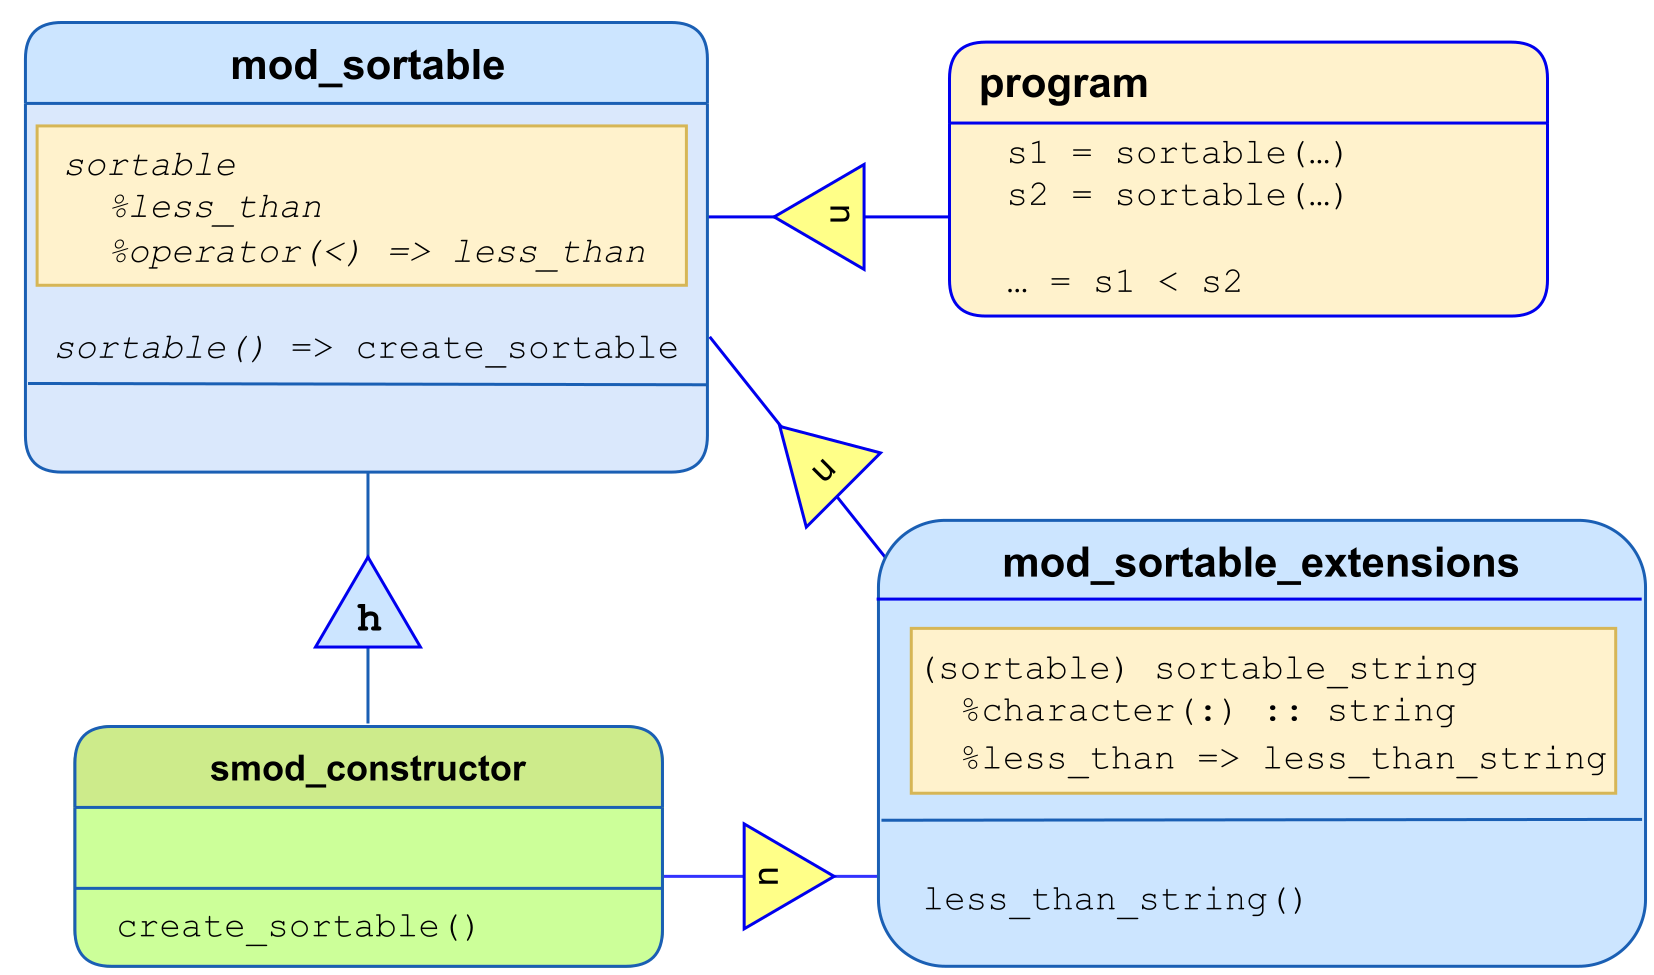
\includegraphics[width=5in,height=\textheight,keepaspectratio]{./images/Dependency_inversion.png}
\caption{Dependencies between program units implementing and using an
interface class}
\end{figure}

The small triangles in the diagram refer to use (``u'') association and
host (``h'') association, respectively. The separation of the
constructor's interface from its implementation leads to avoidance of
circular \texttt{USE} references (the lower two ``u'' triangles in the
diagram).

The compilation order for separate files would be:

\begin{enumerate}
\def\labelenumi{\arabic{enumi}.}
\tightlist
\item
  \texttt{mod\_sortable}
\item
  \texttt{program} and \texttt{mod\_sortable\_extensions}, independently
\item
  \texttt{smod\_constructor}
\end{enumerate}

\section{Performance and ease of use}\label{performance-and-ease-of-use}

\subsection{Functions with
parameters}\label{sec:functions_with_parameters}

\subsubsection{A type definition for invocation of a general
function}\label{a-type-definition-for-invocation-of-a-general-function}

In scientific applications, a commonly occurring requirement is the need
to evaluate functions that depend on additional parameters, apart from
their real-valued argument. For example, an application might need the
value of spherical Bessel function \(x \mapsto j_l(q \, x)\) for
independently specified integer values of \(l\) and real values of
\(q\). More generally, one can consider a real-valued mapping

\(\Re \ni x \mapsto f_\lambda(x) \quad (\lambda \in \Omega)\),

where the parameter value \(\lambda\) can be from some arbitrary set.
This section presents a way for handling this programmatically, using
the object-oriented features of Fortran. We start with the outline for a
type definition of sufficient generality:

\begin{Shaded}
\begin{Highlighting}[]
\DataTypeTok{type}\NormalTok{, }\DataTypeTok{public} \DataTypeTok{::}\NormalTok{ pfunc\_type}
  \DataTypeTok{private}
  \DataTypeTok{procedure(pfunc)}\NormalTok{, }\DataTypeTok{pointer}\NormalTok{, }\DataTypeTok{nopass} \DataTypeTok{::}\NormalTok{ fp }\KeywordTok{=}\OperatorTok{\textgreater{}}\NormalTok{ null()}
\NormalTok{  : }\CommentTok{! shown later}
  \DataTypeTok{class(*)}\NormalTok{, }\DataTypeTok{allocatable} \DataTypeTok{::}\NormalTok{ param}
\KeywordTok{contains}
\NormalTok{  : }\CommentTok{! shown later}
\DataTypeTok{end type}\NormalTok{ pfunc\_type}

\DataTypeTok{abstract} \KeywordTok{interface}
  \KeywordTok{pure} \DataTypeTok{real} \KeywordTok{function}\NormalTok{ pfunc(x, param)}
    \DataTypeTok{real}\NormalTok{, }\DataTypeTok{intent(in)} \DataTypeTok{::}\NormalTok{ x}
    \DataTypeTok{class(*)}\NormalTok{, }\DataTypeTok{intent(in)}\NormalTok{, }\DataTypeTok{optional} \DataTypeTok{::}\NormalTok{ param}
  \KeywordTok{end function}\NormalTok{ pfunc}
\KeywordTok{end interface}
\end{Highlighting}
\end{Shaded}

It supplies

\begin{itemize}
\tightlist
\item
  a \textbf{procedure pointer} component with an abstract interface that
  reflects the above mapping;
\item
  an unlimited polymorphic parameter component, to keep all things in
  one place.
\end{itemize}

Notionally, one could invoke a properly set up \texttt{pfunc\_type}
object through

\begin{Shaded}
\begin{Highlighting}[]
\DataTypeTok{type(pfunc\_type)} \DataTypeTok{::}\NormalTok{ pfunc\_obj}
\DataTypeTok{real} \DataTypeTok{::}\NormalTok{ x}

\NormalTok{pfunc\_obj }\KeywordTok{=}\NormalTok{ pfunc\_type(psin, }\DecValTok{2}\NormalTok{)}
\CommentTok{! definitions of procedure and data object discussed further below}
\NormalTok{x }\KeywordTok{=}\NormalTok{ ...}

\FunctionTok{write(*}\NormalTok{,}\FunctionTok{*)} \StringTok{\textquotesingle{}function value is \textquotesingle{}}\NormalTok{, pfunc\_obj}\OperatorTok{\%}\NormalTok{fp(x, pfunc\_obj}\OperatorTok{\%}\NormalTok{param)}
\end{Highlighting}
\end{Shaded}

Use of a procedure pointer reflects the fact that each
\texttt{pfunc\_type} object will want to associate its individual target
function; this is sometimes also referred to as an \textbf{object-bound
procedure}. The \texttt{nopass} attribute in the type definition is
needed because otherwise (analogous to what we saw for the earlier
type-bound procedure examples), the object through which the invocation
is done would be obliged to appear as a first argument in the abstract
interface \texttt{pfunc}; this would constitute an additional imposition
on the implementation of the supplied functions. On the other hand, the
invocation needs to explicitly specify the \texttt{param} component,
making it a bit unwieldy; the use of \texttt{pfunc\_type} objects will
be simplified as we go on.

\subsubsection{Performance issues arising from object-oriented
programming}\label{performance-issues-arising-from-object-oriented-programming}

Let us look at a target function implementation, in form of a trivial
example \(\sin(\lambda x)\):

\begin{Shaded}
\begin{Highlighting}[]
\KeywordTok{pure} \DataTypeTok{real} \KeywordTok{function}\NormalTok{ psin(x, param)}
  \DataTypeTok{real}\NormalTok{, }\DataTypeTok{intent(in)} \DataTypeTok{::}\NormalTok{ x}
  \DataTypeTok{class(*)}\NormalTok{, }\DataTypeTok{intent(in)}\NormalTok{, }\DataTypeTok{optional} \DataTypeTok{::}\NormalTok{ param}
  \DataTypeTok{real} \DataTypeTok{::}\NormalTok{ factor}
\NormalTok{  factor }\KeywordTok{=} \FloatTok{1.}
  \KeywordTok{if}\NormalTok{ ( }\FunctionTok{present}\NormalTok{(param) ) }\KeywordTok{then}
    \KeywordTok{select type}\NormalTok{ ( param )}
     \KeywordTok{type is}\NormalTok{ (}\DataTypeTok{real}\NormalTok{)}
\NormalTok{      factor }\KeywordTok{=}\NormalTok{ param}
     \KeywordTok{type is}\NormalTok{ (}\DataTypeTok{integer}\NormalTok{)}
\NormalTok{      factor }\KeywordTok{=} \DataTypeTok{real(param)}
    \KeywordTok{end select}
  \KeywordTok{end if}
\NormalTok{  psin }\KeywordTok{=} \BuiltInTok{sin}\NormalTok{(factor}\KeywordTok{*}\NormalTok{x)}
\KeywordTok{end function}\NormalTok{ psin}
\end{Highlighting}
\end{Shaded}

Given that an application is likely to request a large number of
function values, the following effects would ensue once for each
invocation:

\begin{itemize}
\tightlist
\item
  function call overhead, and
\item
  overhead of run-time type resolution.
\end{itemize}

The resulting performance impact is typical for object-oriented designs
that operate in multitudes on small objects. Making use of an
array-based version of the function

\begin{Shaded}
\begin{Highlighting}[]
\KeywordTok{pure} \KeywordTok{function}\NormalTok{ psin\_array(x, param) }\KeywordTok{result}\NormalTok{(r)}
  \DataTypeTok{real}\NormalTok{, }\DataTypeTok{intent(in)} \DataTypeTok{::}\NormalTok{ x(:)}
  \DataTypeTok{real} \DataTypeTok{::}\NormalTok{ r(}\FunctionTok{size}\NormalTok{(x))}
  \DataTypeTok{class(*)}\NormalTok{, }\DataTypeTok{intent(in)}\NormalTok{, }\DataTypeTok{optional} \DataTypeTok{::}\NormalTok{ param}
  \DataTypeTok{real} \DataTypeTok{::}\NormalTok{ factor}
\NormalTok{  factor }\KeywordTok{=} \FloatTok{1.}
  \KeywordTok{if}\NormalTok{ ( }\FunctionTok{present}\NormalTok{(param) ) }\KeywordTok{then}
    \KeywordTok{select type}\NormalTok{ ( param )}
     \KeywordTok{type is}\NormalTok{ (}\DataTypeTok{real}\NormalTok{)}
\NormalTok{      factor }\KeywordTok{=}\NormalTok{ param}
     \KeywordTok{type is}\NormalTok{ (}\DataTypeTok{integer}\NormalTok{)}
\NormalTok{      factor }\KeywordTok{=} \DataTypeTok{real(param)}
    \KeywordTok{end select}
  \KeywordTok{end if}
\NormalTok{  r }\KeywordTok{=} \BuiltInTok{sin}\NormalTok{(factor}\KeywordTok{*}\NormalTok{x)  }\CommentTok{! kernel}
\KeywordTok{end function}\NormalTok{ psin\_array}
\end{Highlighting}
\end{Shaded}

is desirable, since the overheads specified above only arise
\emph{once}, and the actual calculational code (marked ``kernel'' in the
above box) is amenable to array-related compiler optimizations (the
specifics of which depend on both hardware architecture and working set
size).

\subsubsection{Completing the function type
definition}\label{completing-the-function-type-definition}

The aim now is to proceed to a framework that permits to use both the
scalar and the array versions in a uniform way, thereby making life for
the clients that use the framework easy, while enabling performance
where it is needed.

The full definition of \texttt{pfunc\_type}, including its referenced
abstract interfaces, reads

\begin{Shaded}
\begin{Highlighting}[]
\DataTypeTok{type}\NormalTok{, }\DataTypeTok{public} \DataTypeTok{::}\NormalTok{ pfunc\_type}
  \DataTypeTok{private}
  \DataTypeTok{procedure(pfunc)}\NormalTok{, }\DataTypeTok{pointer}\NormalTok{, }\DataTypeTok{nopass} \DataTypeTok{::}\NormalTok{ fp }\KeywordTok{=}\OperatorTok{\textgreater{}}\NormalTok{ null()}
  \DataTypeTok{procedure(pfunc\_array)}\NormalTok{, }\DataTypeTok{pointer}\NormalTok{, }\DataTypeTok{nopass} \DataTypeTok{::}\NormalTok{ fp\_array }\KeywordTok{=}\OperatorTok{\textgreater{}}\NormalTok{ null()}
  \DataTypeTok{class(*)}\NormalTok{, }\DataTypeTok{allocatable} \DataTypeTok{::}\NormalTok{ param}
\KeywordTok{contains}
  \DataTypeTok{procedure}\NormalTok{, }\DataTypeTok{pass}\NormalTok{, }\DataTypeTok{private}\NormalTok{, }\DataTypeTok{non\_overridable} \DataTypeTok{::}\NormalTok{ f\_scalar, f\_array}
  \DataTypeTok{generic} \DataTypeTok{::}\NormalTok{ f }\KeywordTok{=}\OperatorTok{\textgreater{}}\NormalTok{ f\_scalar, f\_array}
\DataTypeTok{end type}\NormalTok{ pfunc\_type}

\DataTypeTok{abstract} \KeywordTok{interface}
  \KeywordTok{pure} \DataTypeTok{real} \KeywordTok{function}\NormalTok{ pfunc(x, param)}
    \DataTypeTok{real}\NormalTok{, }\DataTypeTok{intent(in)} \DataTypeTok{::}\NormalTok{ x}
    \DataTypeTok{class(*)}\NormalTok{, }\DataTypeTok{intent(in)}\NormalTok{, }\DataTypeTok{optional} \DataTypeTok{::}\NormalTok{ param}
  \KeywordTok{end function}\NormalTok{ pfunc}
  \KeywordTok{pure} \KeywordTok{function}\NormalTok{ pfunc\_array(x, param) }\KeywordTok{result}\NormalTok{(r)}
    \DataTypeTok{real}\NormalTok{, }\DataTypeTok{intent(in)} \DataTypeTok{::}\NormalTok{ x(:)}
    \DataTypeTok{real} \DataTypeTok{::}\NormalTok{ r(}\FunctionTok{size}\NormalTok{(x))}
    \DataTypeTok{class(*)}\NormalTok{, }\DataTypeTok{intent(in)}\NormalTok{, }\DataTypeTok{optional} \DataTypeTok{::}\NormalTok{ param}
  \KeywordTok{end function}\NormalTok{ pfunc\_array}
\KeywordTok{end interface}
\end{Highlighting}
\end{Shaded}

Because we now have two procedure pointers in the type (only one of
which is used in each given object), it is advantageous to provide a
generic type-bound procedure \texttt{f} as a front end for ease of use.
The specifics \texttt{f\_scalar} and \texttt{f\_array} for this read

\begin{Shaded}
\begin{Highlighting}[]
\DataTypeTok{real} \KeywordTok{function}\NormalTok{ f\_scalar(this, x)}
  \DataTypeTok{class(pfunc\_type)}\NormalTok{, }\DataTypeTok{intent(in)} \DataTypeTok{::}\NormalTok{ this}
  \DataTypeTok{real}\NormalTok{, }\DataTypeTok{intent(in)} \DataTypeTok{::}\NormalTok{ x}

  \KeywordTok{if}\NormalTok{ ( }\FunctionTok{associated}\NormalTok{(this}\OperatorTok{\%}\NormalTok{fp) ) }\KeywordTok{then}
\NormalTok{    f\_scalar }\KeywordTok{=}\NormalTok{ this}\OperatorTok{\%}\NormalTok{fp(x, this}\OperatorTok{\%}\NormalTok{param)}
  \KeywordTok{else} \KeywordTok{if}\NormalTok{ ( }\FunctionTok{associated}\NormalTok{(this}\OperatorTok{\%}\NormalTok{fp\_array) ) }\KeywordTok{then}
    \KeywordTok{associate}\NormalTok{ ( f\_array }\KeywordTok{=}\OperatorTok{\textgreater{}}\NormalTok{ this}\OperatorTok{\%}\NormalTok{fp\_array(}\KeywordTok{[}\NormalTok{x}\KeywordTok{]}\NormalTok{, this}\OperatorTok{\%}\NormalTok{param) )}
\NormalTok{      f\_scalar }\KeywordTok{=}\NormalTok{ f\_array(}\DecValTok{1}\NormalTok{)}
    \KeywordTok{end associate}
  \KeywordTok{else}
\NormalTok{    error }\KeywordTok{stop} \StringTok{\textquotesingle{}pfunc\_type callback: uninitialized object\textquotesingle{}}
  \KeywordTok{end if}
\KeywordTok{end function}\NormalTok{ f\_scalar}
\KeywordTok{function}\NormalTok{ f\_array(this, x) }\KeywordTok{result}\NormalTok{(r)}
  \DataTypeTok{class(pfunc\_type)}\NormalTok{, }\DataTypeTok{intent(in)} \DataTypeTok{::}\NormalTok{ this}
  \DataTypeTok{real}\NormalTok{, }\DataTypeTok{intent(in)} \DataTypeTok{::}\NormalTok{ x(:)}
  \DataTypeTok{real} \DataTypeTok{::}\NormalTok{ r(}\FunctionTok{size}\NormalTok{(x))}

  \CommentTok{! note that support for the scalar version is omitted here, since}
  \CommentTok{! the procedure call overhead, including type resolution, would}
  \CommentTok{! significantly impact performance.}
  \KeywordTok{if}\NormalTok{ ( }\FunctionTok{associated}\NormalTok{(this}\OperatorTok{\%}\NormalTok{fp\_array) ) }\KeywordTok{then}
\NormalTok{    r }\KeywordTok{=}\NormalTok{ this}\OperatorTok{\%}\NormalTok{fp\_array(x, this}\OperatorTok{\%}\NormalTok{param)}
  \KeywordTok{else}
\NormalTok{    error }\KeywordTok{stop} \StringTok{\textquotesingle{}pfunc\_type callback: uninitialized object\textquotesingle{}}
  \KeywordTok{end if}
\KeywordTok{end function}\NormalTok{ f\_array}
\end{Highlighting}
\end{Shaded}

The only way to invoke one of these (in a use association context) is
via the generic name, since the specific type-bound procedures have the
\texttt{private} attribute; note that \texttt{pfunc\_type} is not
designed for being extended. Disambiguation is by rank of \texttt{x}.

The structure constructor for the type is overloaded

\begin{Shaded}
\begin{Highlighting}[]
\KeywordTok{interface}\NormalTok{ pfunc\_type}
  \KeywordTok{module procedure}\NormalTok{ create\_pfunc\_type}
  \KeywordTok{module procedure}\NormalTok{ create\_pfunc\_type\_array}
\KeywordTok{end interface}\NormalTok{ pfunc\_type}
\end{Highlighting}
\end{Shaded}

with the following specific functions:

\begin{Shaded}
\begin{Highlighting}[]
\DataTypeTok{type(pfunc\_type)} \KeywordTok{function}\NormalTok{ create\_pfunc\_type(fp, param)}
  \DataTypeTok{procedure(pfunc)} \DataTypeTok{::}\NormalTok{ fp}
  \DataTypeTok{class(*)}\NormalTok{, }\DataTypeTok{intent(in)}\NormalTok{, }\DataTypeTok{optional} \DataTypeTok{::}\NormalTok{ param}
\NormalTok{  create\_pfunc\_type}\OperatorTok{\%}\NormalTok{fp }\KeywordTok{=}\OperatorTok{\textgreater{}}\NormalTok{ fp}
  \KeywordTok{if}\NormalTok{ ( }\FunctionTok{present}\NormalTok{(param) ) }\KeywordTok{then}
    \KeywordTok{allocate}\NormalTok{(create\_pfunc\_type}\OperatorTok{\%}\NormalTok{param, source}\KeywordTok{=}\NormalTok{param)}
  \KeywordTok{end if}
\KeywordTok{end function}\NormalTok{ create\_pfunc\_type}
\DataTypeTok{type(pfunc\_type)} \KeywordTok{function}\NormalTok{ create\_pfunc\_type\_array(fp\_array, param)}
  \DataTypeTok{procedure(pfunc\_array)} \DataTypeTok{::}\NormalTok{ fp\_array}
  \DataTypeTok{class(*)}\NormalTok{, }\DataTypeTok{intent(in)}\NormalTok{, }\DataTypeTok{optional} \DataTypeTok{::}\NormalTok{ param}
\NormalTok{  create\_pfunc\_type\_array}\OperatorTok{\%}\NormalTok{fp\_array }\KeywordTok{=}\OperatorTok{\textgreater{}}\NormalTok{ fp\_array}
  \KeywordTok{if}\NormalTok{ ( }\FunctionTok{present}\NormalTok{(param) ) }\KeywordTok{then}
    \KeywordTok{allocate}\NormalTok{(create\_pfunc\_type\_array}\OperatorTok{\%}\NormalTok{param, source}\KeywordTok{=}\NormalTok{param)}
  \KeywordTok{end if}
\KeywordTok{end function}\NormalTok{ create\_pfunc\_type\_array}
\end{Highlighting}
\end{Shaded}

Disambiguation is possible due to the sufficiently different interfaces
of the procedure arguments.\footnote{Brad Richardson
  \href{https://fortran-lang.discourse.group/t/baders-draft-about-oop-and-fortran-bader-intended-for-wikipedia/8539/3}{comments}
  the two functions are \emph{sufficiently different} only because their
  results differ in rank. This pattern does not necessarily work in the
  general case, i.e.~that the procedures are not both functions with
  different type, kind or rank of their results.

  More generally, referring to section 15.4.3.4.5 \emph{Restrictions on
  generic declarations} of the current Fortran 2023 standard (see for
  instance \href{https://j3-fortran.org/doc/year/23/23-007r1.pdf}{draft
  23-007r1.pdf}, page 316)

  \begin{quote}
  Two dummy arguments are distinguishable if

  \begin{itemize}
  \tightlist
  \item
    one is a procedure and the other is a data object,
  \item
    they are both data objects or known to be functions, and neither is
    TKR compatible with the other, one has the ALLOCATABLE attribute and
    the other has the POINTER attribute and not the INTENT (IN)
    attribute, or
  \item
    one is a function with nonzero rank and the other is not known to be
    a function.
  \end{itemize}
  \end{quote}}

\subsubsection{Using the function type}\label{using-the-function-type}

With the already-shown implementations for the target functions
\texttt{psin} and \texttt{psin\_array}, using this framework is
illustrated by the following:

\begin{Shaded}
\begin{Highlighting}[]
\DataTypeTok{type(pfunc\_type)} \DataTypeTok{::}\NormalTok{ pfunc\_obj}
\DataTypeTok{real}\NormalTok{, }\DataTypeTok{parameter} \DataTypeTok{::}\NormalTok{ piby4 }\KeywordTok{=} \BuiltInTok{atan}\NormalTok{(}\FloatTok{1.0}\NormalTok{), }\KeywordTok{\&}
\NormalTok{  piby4\_arr(}\DecValTok{4}\NormalTok{) }\KeywordTok{=} \KeywordTok{[}\NormalTok{ piby4, }\FloatTok{2.}\KeywordTok{*}\NormalTok{piby4, }\FloatTok{3.}\KeywordTok{*}\NormalTok{piby4, }\FloatTok{4.}\KeywordTok{*}\NormalTok{piby4 }\KeywordTok{]}

\NormalTok{pfunc\_obj }\KeywordTok{=}\NormalTok{ pfunc\_type(psin, }\FloatTok{2.}\NormalTok{)}
\FunctionTok{write(*}\NormalTok{,}\FunctionTok{*)}\NormalTok{ pfunc\_obj}\OperatorTok{\%}\NormalTok{f(piby4)}

\NormalTok{pfunc\_obj }\KeywordTok{=}\NormalTok{ pfunc\_type(psin)}
\FunctionTok{write(*}\NormalTok{,}\FunctionTok{*)}\NormalTok{ pfunc\_obj}\OperatorTok{\%}\NormalTok{f(piby4)}

\NormalTok{pfunc\_obj }\KeywordTok{=}\NormalTok{ pfunc\_type(psin\_array, }\FloatTok{2.}\NormalTok{)}
\FunctionTok{write(*}\NormalTok{,}\FunctionTok{*)}\NormalTok{ pfunc\_obj}\OperatorTok{\%}\NormalTok{f(piby4\_arr)}
\end{Highlighting}
\end{Shaded}

Omitting a \texttt{param} in a constructor is fine, as long as the
target functions cater for the dummy argument's non-presence.

\emph{Hint:} The framework's implementation makes use of the fact that
an unallocated actual argument associated with an \texttt{optional}
dummy argument is considered not present. Once conditional expressions
are implemented in compilers, the code will be appropriately reworked,
since use of this feature is recommended against.

\subsection{Arrays of structures versus structures of
arrays}\label{arrays-of-structures-versus-structures-of-arrays}

Returning to our earlier example type body, the next idea would be to
simulate the dynamics of a large ensemble of bodies. A procedure

\begin{Shaded}
\begin{Highlighting}[]
\KeywordTok{subroutine}\NormalTok{ propagate(bodies, delta\_t, force\_field)}
  \DataTypeTok{type(body)}\NormalTok{, }\DataTypeTok{intent(inout)} \DataTypeTok{::}\NormalTok{ bodies(:)}
  \DataTypeTok{real}\NormalTok{, }\DataTypeTok{intent(in)} \DataTypeTok{::}\NormalTok{ delta\_t}
  \DataTypeTok{type(field\_type)}\NormalTok{, }\DataTypeTok{intent(in)} \DataTypeTok{::}\NormalTok{ force\_field}
\NormalTok{  :}
\KeywordTok{end subroutine}
\end{Highlighting}
\end{Shaded}

might be supplied that modifies the components of all ensemble members,
for example as follows:

\begin{itemize}
\tightlist
\item
  \texttt{\%pos} \(\longrightarrow\)
  \texttt{\%pos\ +\ delta\_t\ *\ \%vel}
\item
  \texttt{\%vel} \(\longrightarrow\)
  \texttt{\%vel\ +\ delta\_t\ *\ force\ /\ \%mass}
\end{itemize}

where \texttt{force} results from evaluating \texttt{force\_field} at
the position of the ensemble member.

\subsection{Comments on further language
features}\label{comments-on-further-language-features}

\subsubsection{Variations on the passed
object}\label{variations-on-the-passed-object}

All examples for type-bound procedures given up to now have the property
that the invoking object itself is passed as the first argument to the
bound procedure. However, this default behaviour can be modified by the
programmer

\begin{itemize}
\tightlist
\item
  either declaring the binding with a \texttt{pass} attribute that
  references the specific (and of course appropriately declared)
  procedure argument the object of the bound type should be passed to,
\item
  or declaring the binding with a \texttt{nopass} attribute, in which
  case the object is not (implicitly) passed to the procedure at all in
  a TBP invocation.
\end{itemize}

\end{document}
